\documentclass[11pt,a4paper]{ctexart}

\usepackage[margin=1.8cm]{geometry}
\usepackage{graphicx}
\usepackage{subcaption}
\usepackage{booktabs}
\usepackage{array}
\usepackage{amsmath}
\usepackage{hyperref}
\usepackage{xcolor}
\usepackage{enumitem}
\usepackage{float}
\usepackage{caption}
\usepackage{tcolorbox}
\usepackage{listings}
\usepackage{tikz}
\usetikzlibrary{arrows.meta,positioning}

\graphicspath{{./}}
\hypersetup{
  colorlinks=true,
  linkcolor=black,
  urlcolor=blue,
  citecolor=black
}

\definecolor{paperblue}{RGB}{35,70,120}
\definecolor{papergray}{RGB}{245,246,248}
\definecolor{darkgray}{RGB}{70,70,70}
\definecolor{softblue}{RGB}{232,239,249}
\definecolor{softgreen}{RGB}{234,247,239}
\definecolor{softorange}{RGB}{252,242,226}

\captionsetup{font=small,labelfont=bf}
\setlist[itemize]{leftmargin=1.4em,itemsep=0.2em,topsep=0.2em}
\setlist[enumerate]{leftmargin=1.6em,itemsep=0.2em,topsep=0.2em}

\lstset{
  basicstyle=\ttfamily\small,
  breaklines=true,
  frame=single,
  backgroundcolor=\color{papergray},
  rulecolor=\color{papergray}
}

\newcommand{\code}[1]{\texttt{\detokenize{#1}}}
\newcommand{\figpath}[1]{\texttt{\detokenize{#1}}}

\tikzset{
  frameworkbox/.style={
    draw=paperblue,
    rounded corners=1.5mm,
    line width=0.8pt,
    align=center,
    minimum height=8mm,
    inner xsep=4mm,
    inner ysep=2mm,
    font=\small
  },
  frameworkroot/.style={frameworkbox, fill=softblue, font=\small\bfseries},
  frameworkcont/.style={frameworkbox, fill=softgreen},
  frameworkdisc/.style={frameworkbox, fill=softorange},
  frameworkarrow/.style={-Stealth, line width=0.8pt, draw=darkgray}
}

\title{\vspace{-1.2cm}\textbf{Flow Matching 与 Diffusion 项目阶段总结}\\
\large 从课程 Lab 到类别条件图像生成展示项目}
\author{RectifiedFlow-Lab}
\date{\today}

\begin{document}
\maketitle

\begin{tcolorbox}[colback=papergray,colframe=paperblue,title=\textbf{项目结论},arc=1mm]
本项目包含两条主线：第一条是课程式 Lab，覆盖 ODE/SDE、Flow Matching、DDPM、CFG、Mini-DiT 与离散扩散；第二条是展示项目，从 CIFAR-10 U-Net Rectified Flow baseline 出发，经过采样消融、质量提升、DDPM/DDIM 强 baseline、EDM 与 Visual64 扩展，最终得到可展示的类别条件生成结果。当前最强 CIFAR-10 定量结果为 DDPM/DDIM cosine v-prediction U-Net：FID 13.37，IS 5.29；最清晰的视觉展示来自 Visual64 Pets EDM。
\end{tcolorbox}

\tableofcontents
\newpage

\section{总体架构}

项目目标不是只训练一个模型，而是把“理论路径、预测目标、网络结构、采样器、消融分析、展示结果”串成闭环。核心统一视角为
\[
  x_0 \sim p_0,\qquad x_1 \sim p_{\mathrm{data}},\qquad
  x_t=(1-t)x_0+t x_1,\qquad
  v_\theta(x_t,t,y)\approx x_1-x_0.
\]
这一路径解释了 Flow Matching 和 Rectified Flow；DDPM/EDM 分支则作为更强的图像质量 baseline，用于判断“问题来自理论目标、采样器，还是工程配置”。

\begin{figure}[H]
  \centering
  \resizebox{0.96\linewidth}{!}{
  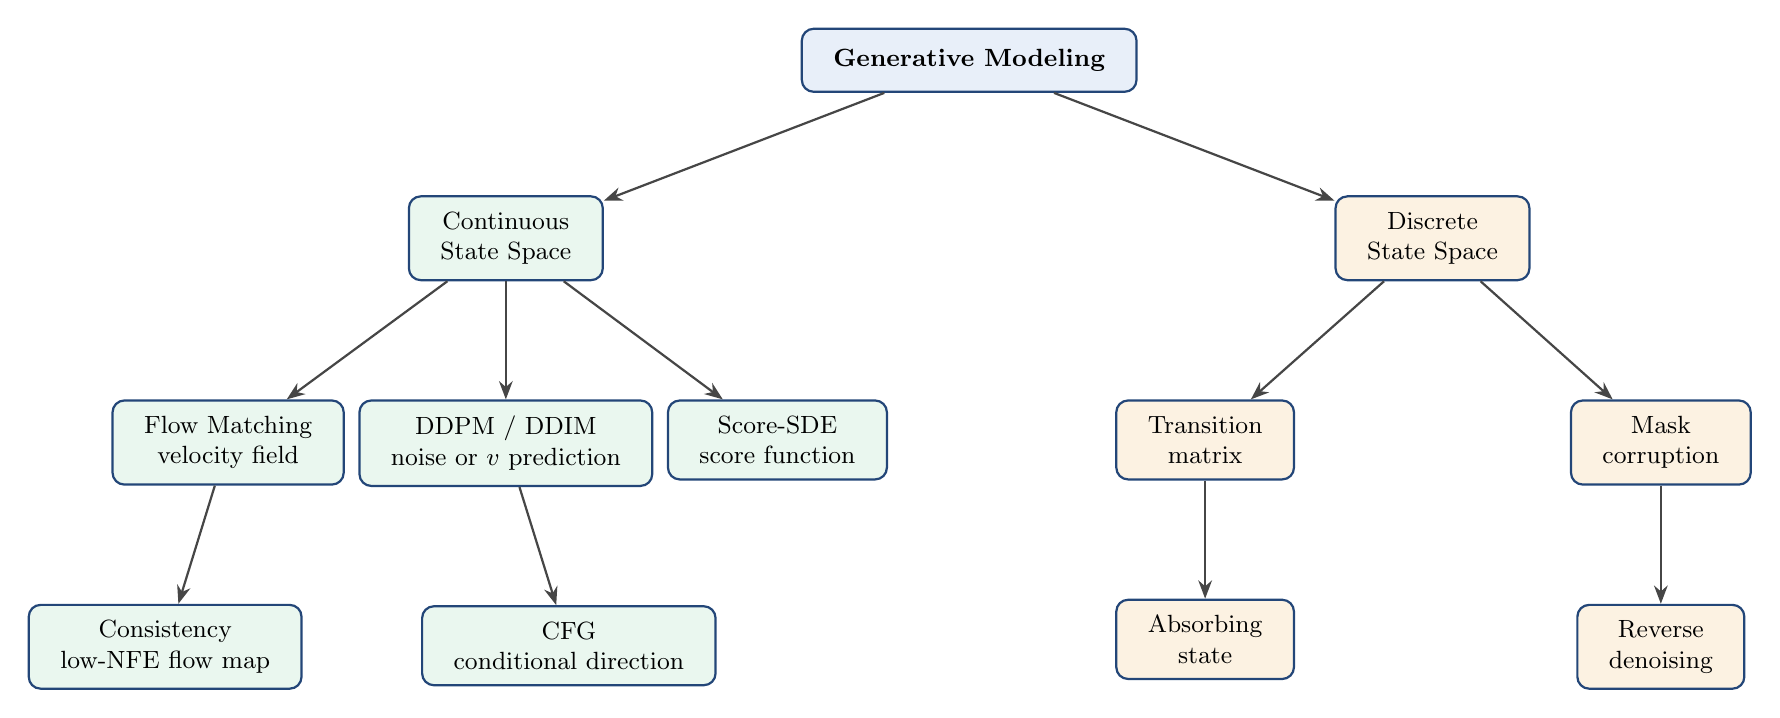
\begin{tikzpicture}[node distance=13mm and 13mm]
    \node[frameworkroot] (gen) {Generative Modeling};

    \node[frameworkcont, below left=13mm and 25mm of gen] (cont) {Continuous\\State Space};
    \node[frameworkdisc, below right=13mm and 25mm of gen] (disc) {Discrete\\State Space};

    \node[frameworkcont, below left=15mm and 8mm of cont] (fm) {Flow Matching\\velocity field};
    \node[frameworkcont, below=15mm of cont] (ddpm) {DDPM / DDIM\\noise or $v$ prediction};
    \node[frameworkcont, below right=15mm and 8mm of cont] (score) {Score-SDE\\score function};

    \node[frameworkdisc, below left=15mm and 5mm of disc] (trans) {Transition\\matrix};
    \node[frameworkdisc, below right=15mm and 5mm of disc] (mask) {Mask\\corruption};

    \node[frameworkcont, below=15mm of ddpm, xshift=8mm] (cfg) {CFG\\conditional direction};
    \node[frameworkcont, below=15mm of fm, xshift=-8mm] (cons) {Consistency\\low-NFE flow map};

    \node[frameworkdisc, below=15mm of trans] (absorb) {Absorbing\\state};
    \node[frameworkdisc, below=15mm of mask] (reverse) {Reverse\\denoising};

    \draw[frameworkarrow] (gen) -- (cont);
    \draw[frameworkarrow] (gen) -- (disc);

    \draw[frameworkarrow] (cont) -- (fm);
    \draw[frameworkarrow] (cont) -- (ddpm);
    \draw[frameworkarrow] (cont) -- (score);

    \draw[frameworkarrow] (disc) -- (trans);
    \draw[frameworkarrow] (disc) -- (mask);

    \draw[frameworkarrow] (ddpm) -- (cfg);
    \draw[frameworkarrow] (fm) -- (cons);

    \draw[frameworkarrow] (trans) -- (absorb);
    \draw[frameworkarrow] (mask) -- (reverse);
  \end{tikzpicture}}
  \caption{统一理论框架：连续扩散、Flow Matching、快速采样与离散扩散都可以放入概率路径和反向生成过程的视角下。图中箭头只表示直接依赖关系，避免跨层连线造成语义混淆。}
\end{figure}

\section{第一部分：课程 Lab 总结}

\subsection{Lab 1：概率路径、ODE 与 SDE}

\paragraph{理论基础}
Lab 1 建立生成模型的基础语言：从简单分布到数据分布的概率路径、确定性 ODE 轨迹，以及随机 SDE 轨迹。ODE 强调确定性流映射，SDE 强调布朗运动和噪声驱动的分布演化。

\paragraph{关键代码}
\begin{itemize}
  \item \code{src/toy_data.py}：构造二维 toy distribution。
  \item \code{src/ode.py}：Euler ODE 积分与轨迹模拟。
  \item \code{src/sde.py}：Brownian motion 和 SDE 采样。
  \item \code{labs/lab1/run_probability_path.py}、\code{labs/lab1/run_ode_sde.py}：实验入口。
\end{itemize}

\begin{figure}[H]
  \centering
  \begin{subfigure}{0.32\linewidth}
    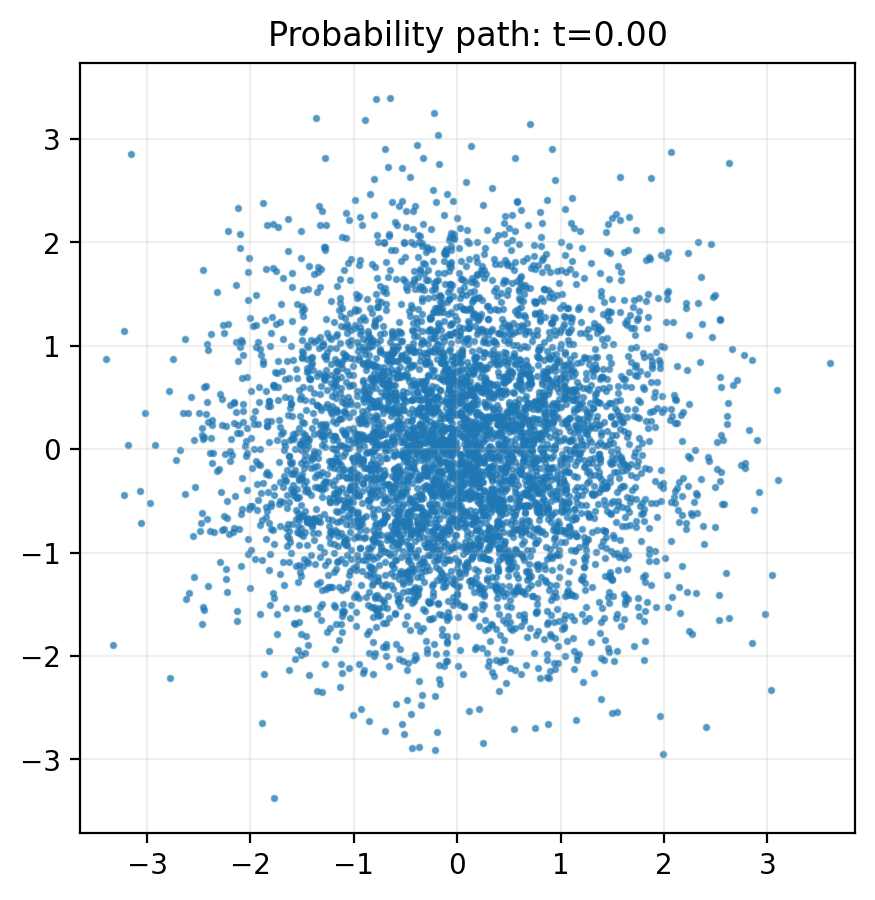
\includegraphics[width=\linewidth]{figures/stage1/probability_path_t_0.00.png}
    \caption{$t=0$}
  \end{subfigure}
  \begin{subfigure}{0.32\linewidth}
    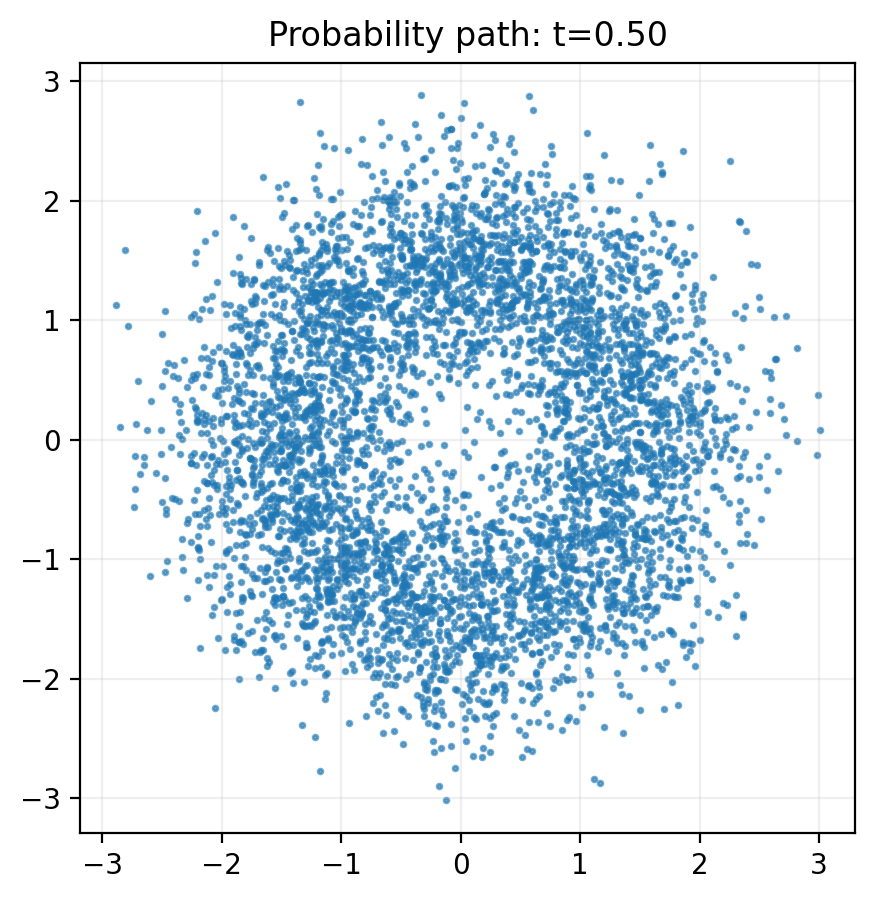
\includegraphics[width=\linewidth]{figures/stage1/probability_path_t_0.50.png}
    \caption{$t=0.5$}
  \end{subfigure}
  \begin{subfigure}{0.32\linewidth}
    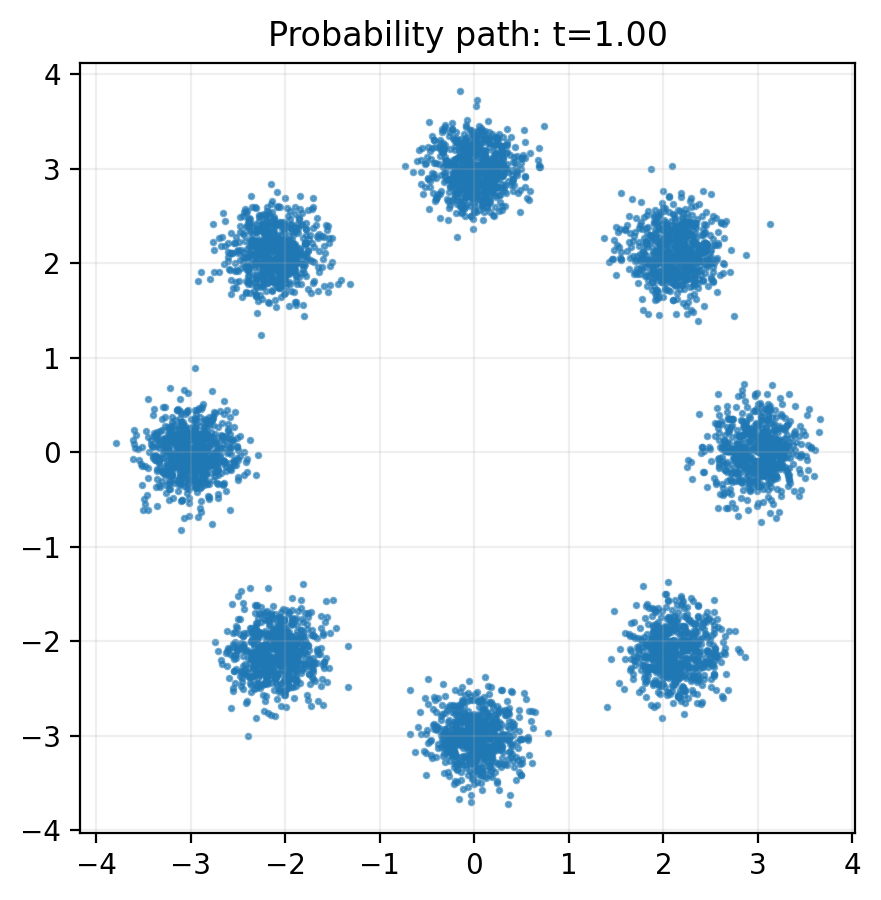
\includegraphics[width=\linewidth]{figures/stage1/probability_path_t_1.00.png}
    \caption{$t=1$}
  \end{subfigure}
  \caption{概率路径从简单先验逐渐移动到目标数据分布。}
\end{figure}

\begin{figure}[H]
  \centering
  \begin{subfigure}{0.48\linewidth}
    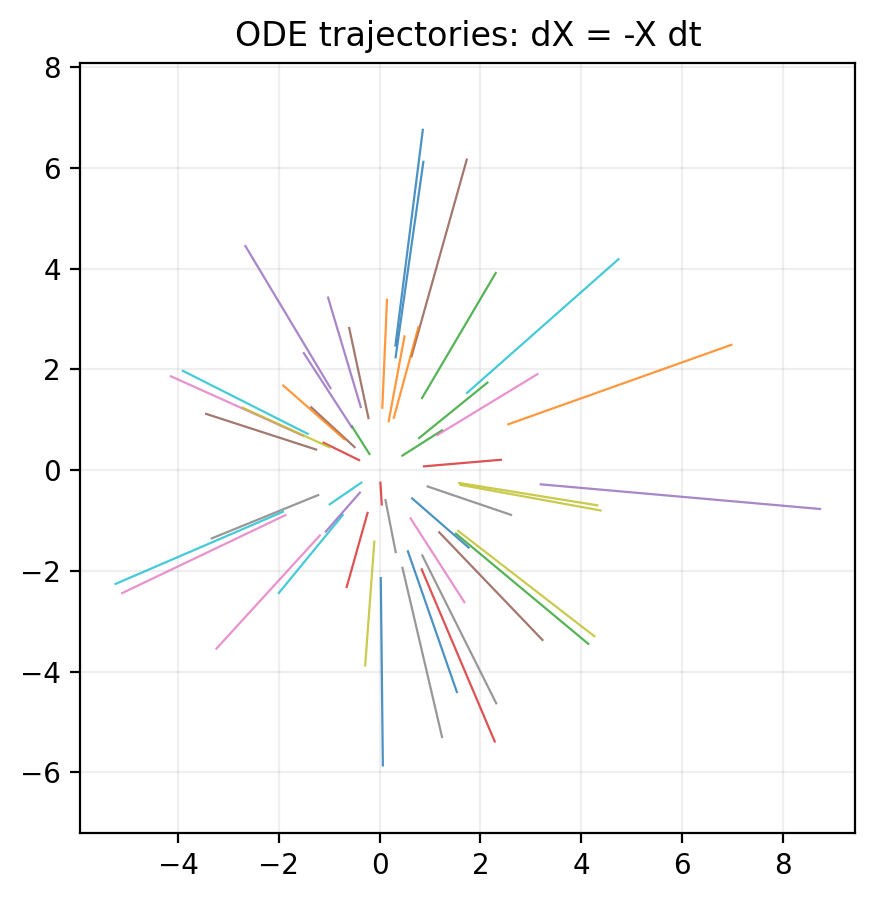
\includegraphics[width=\linewidth]{figures/stage1/ode_trajectories.png}
    \caption{ODE 轨迹}
  \end{subfigure}
  \begin{subfigure}{0.48\linewidth}
    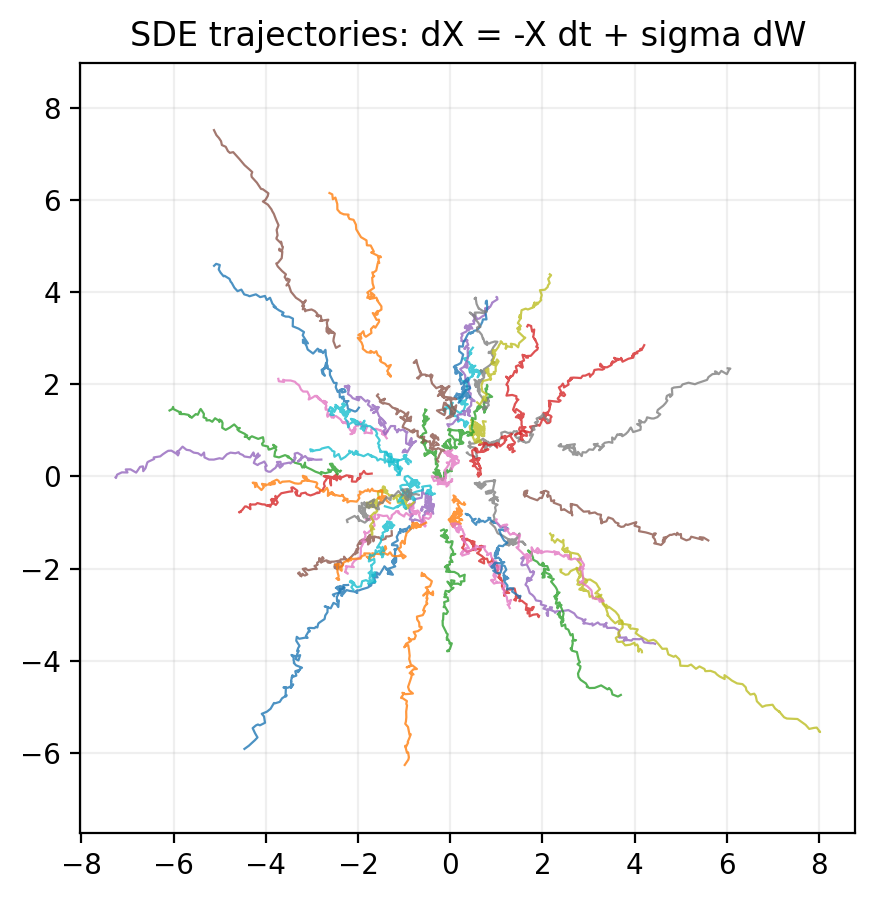
\includegraphics[width=\linewidth]{figures/stage1/sde_trajectories.png}
    \caption{SDE 轨迹}
  \end{subfigure}
  \caption{ODE 与 SDE 的差异：ODE 轨迹平滑确定，SDE 轨迹包含随机扰动。}
\end{figure}

\paragraph{结果分析}
概率路径图说明了生成模型的根本任务：把 $p_0$ 运输到 $p_{\mathrm{data}}$。ODE/SDE 对比说明采样算法既可以通过确定性速度场完成，也可以通过含噪反向过程完成。这为后续 Flow Matching 与 DDPM 的区别打下基础。

\subsection{Lab 2：二维 Flow Matching}

\paragraph{理论基础}
Flow Matching 学习条件速度场，而不是逐步预测噪声。在线性路径下：
\[
  x_t=(1-t)x_0+t x_1,\qquad u_t=x_1-x_0,\qquad
  \mathcal{L}=\|v_\theta(x_t,t)-u_t\|_2^2.
\]
采样时解 ODE：$\frac{dx}{dt}=v_\theta(x,t)$。

\paragraph{关键代码}
\begin{itemize}
  \item \code{src/flow_matching.py}：构造 $(x_0,t,x_t,u_t)$ 与 FM loss。
  \item \code{src/mlp.py}：二维速度场 MLP。
  \item \code{src/samplers.py}：Euler、Heun 采样器。
  \item \code{labs/lab2/run_2d_flow_matching.py}：训练、采样与可视化。
\end{itemize}

\begin{figure}[H]
  \centering
  \begin{subfigure}{0.32\linewidth}
    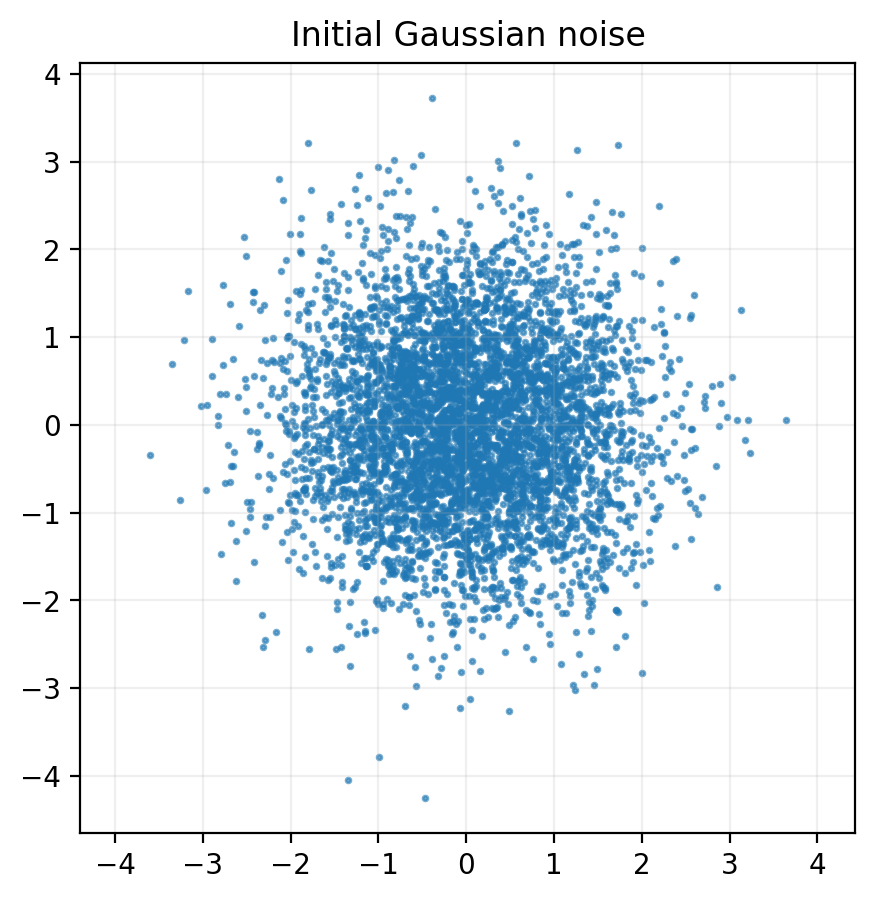
\includegraphics[width=\linewidth]{figures/stage2/initial_noise.png}
    \caption{初始噪声}
  \end{subfigure}
  \begin{subfigure}{0.32\linewidth}
    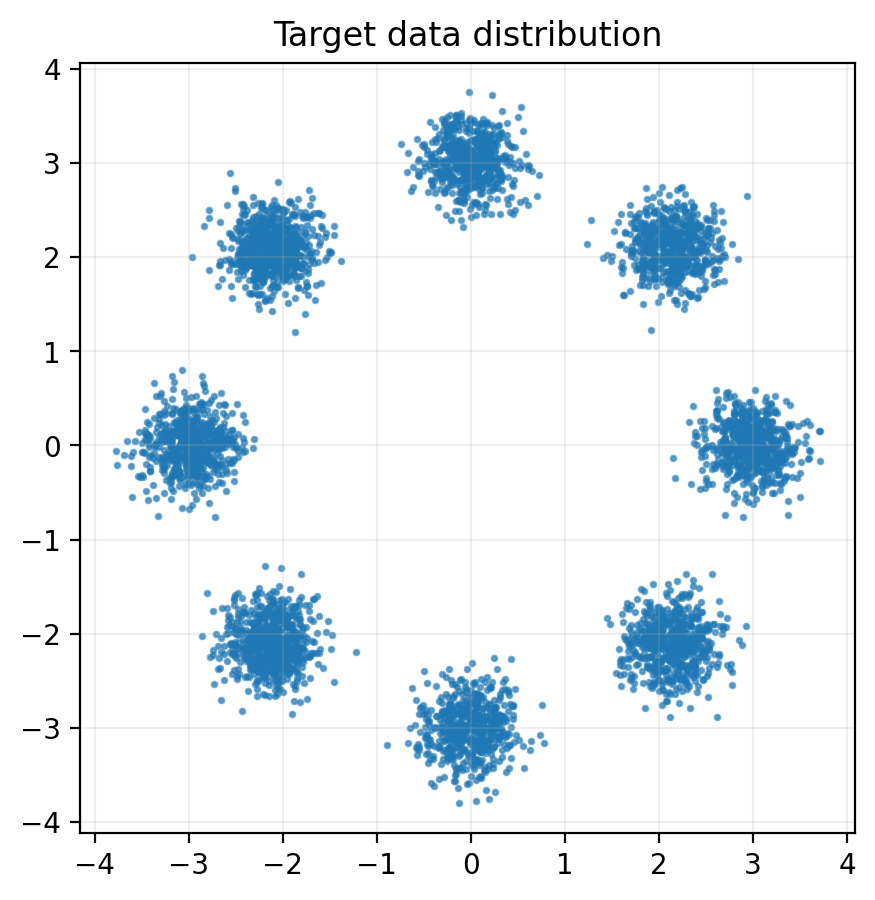
\includegraphics[width=\linewidth]{figures/stage2/target_data.png}
    \caption{目标数据}
  \end{subfigure}
  \begin{subfigure}{0.32\linewidth}
    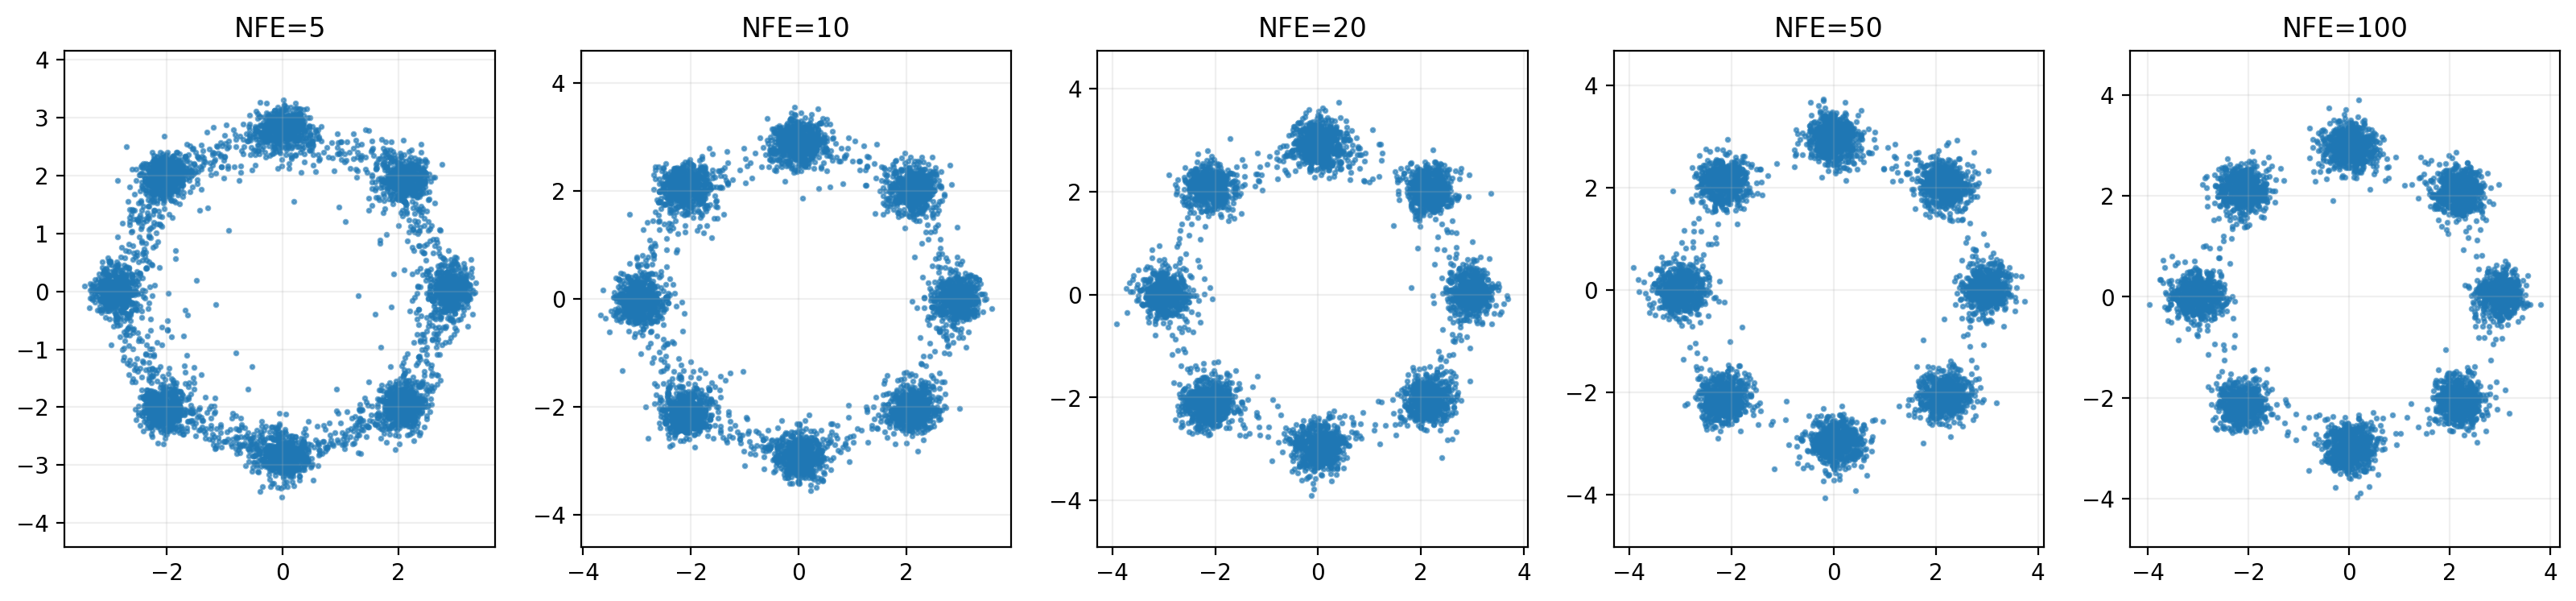
\includegraphics[width=\linewidth]{figures/stage2/fm_samples_nfe_compare.png}
    \caption{NFE 对比}
  \end{subfigure}
  \caption{二维 Flow Matching 从噪声生成目标分布，并通过 NFE 观察积分步数对质量的影响。}
\end{figure}

\begin{figure}[H]
  \centering
  \begin{subfigure}{0.48\linewidth}
    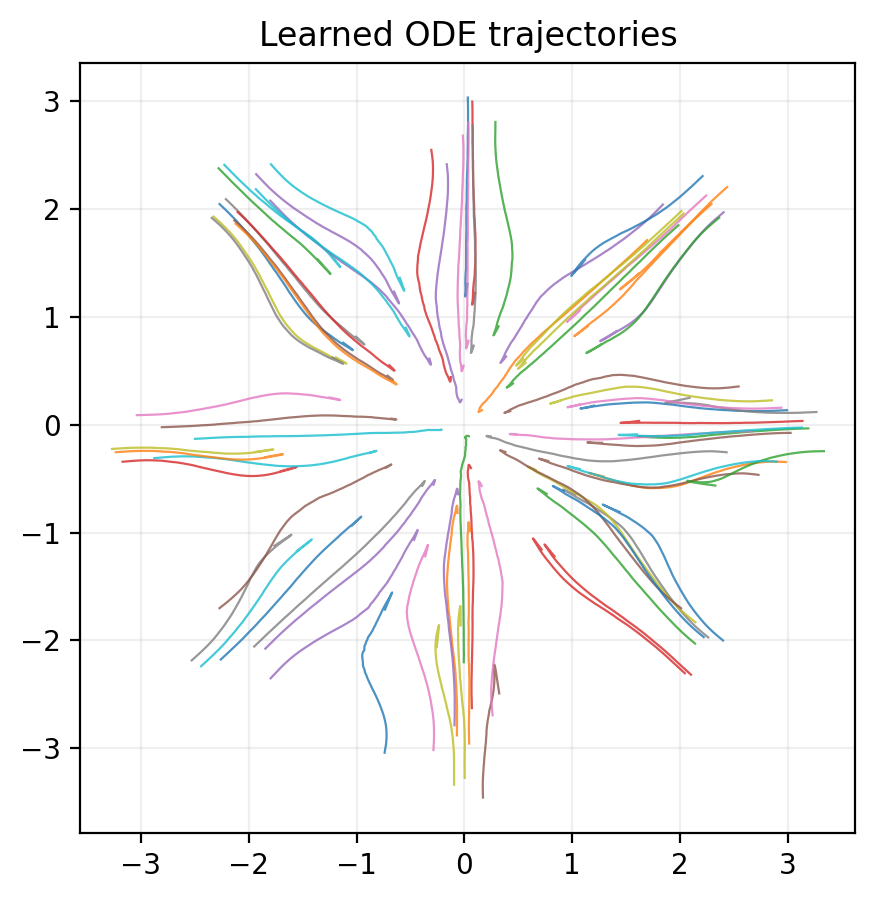
\includegraphics[width=\linewidth]{figures/stage2/fm_trajectories.png}
    \caption{采样轨迹}
  \end{subfigure}
  \begin{subfigure}{0.48\linewidth}
    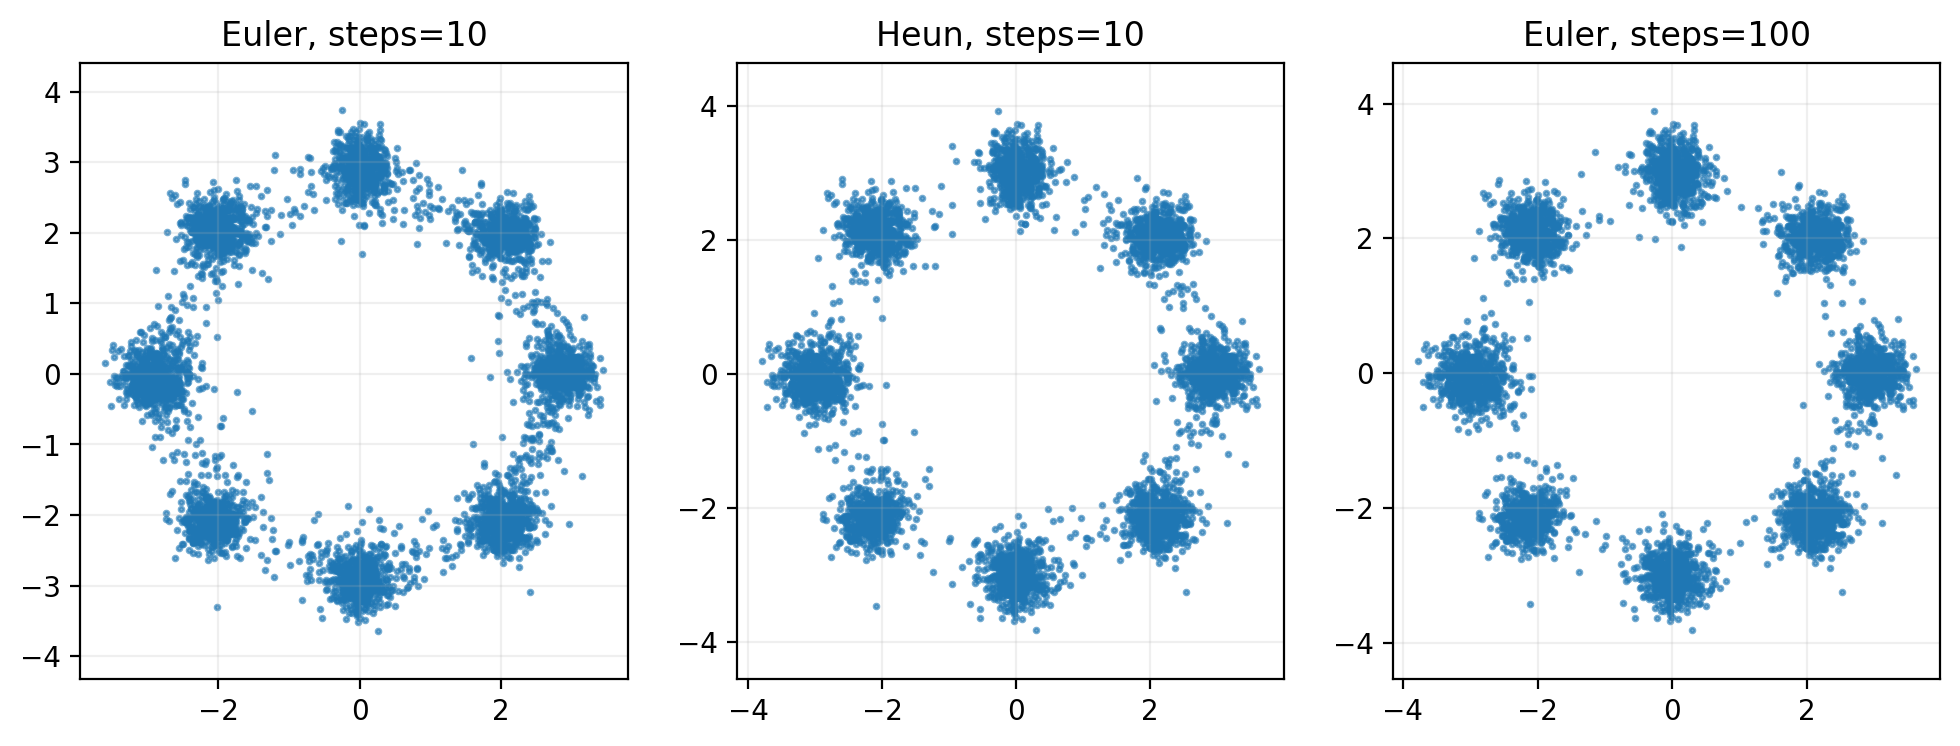
\includegraphics[width=\linewidth]{figures/stage2/fm_euler_vs_heun.png}
    \caption{Euler 与 Heun}
  \end{subfigure}
  \caption{轨迹和求解器对比展示了 ODE sampler 对最终生成分布的影响。}
\end{figure}

\paragraph{结果分析}
NFE 增大时，样本更接近目标分布；Heun 在低步数下通常比 Euler 更稳定。该 Lab 直接对应后续 CIFAR-10 项目中的 NFE、solver 和 runtime 消融。

\subsection{Lab 3：Score Matching 与 DDPM}

\paragraph{理论基础}
DDPM 通过前向加噪 $q(x_t|x_0)$ 和反向去噪 $p_\theta(x_{t-1}|x_t)$ 学习生成过程。训练常用噪声预测：
\[
  x_t=\sqrt{\bar{\alpha}_t}x_0+\sqrt{1-\bar{\alpha}_t}\epsilon,\qquad
  \mathcal{L}=\|\epsilon_\theta(x_t,t)-\epsilon\|_2^2.
\]

\paragraph{关键代码}
\begin{itemize}
  \item \code{src/diffusion.py}：DDPM schedule、前向加噪与反向采样。
  \item \code{labs/lab2/run_2d_ddpm.py}：二维 DDPM 训练与采样。
\end{itemize}

\begin{figure}[H]
  \centering
  \begin{subfigure}{0.32\linewidth}
    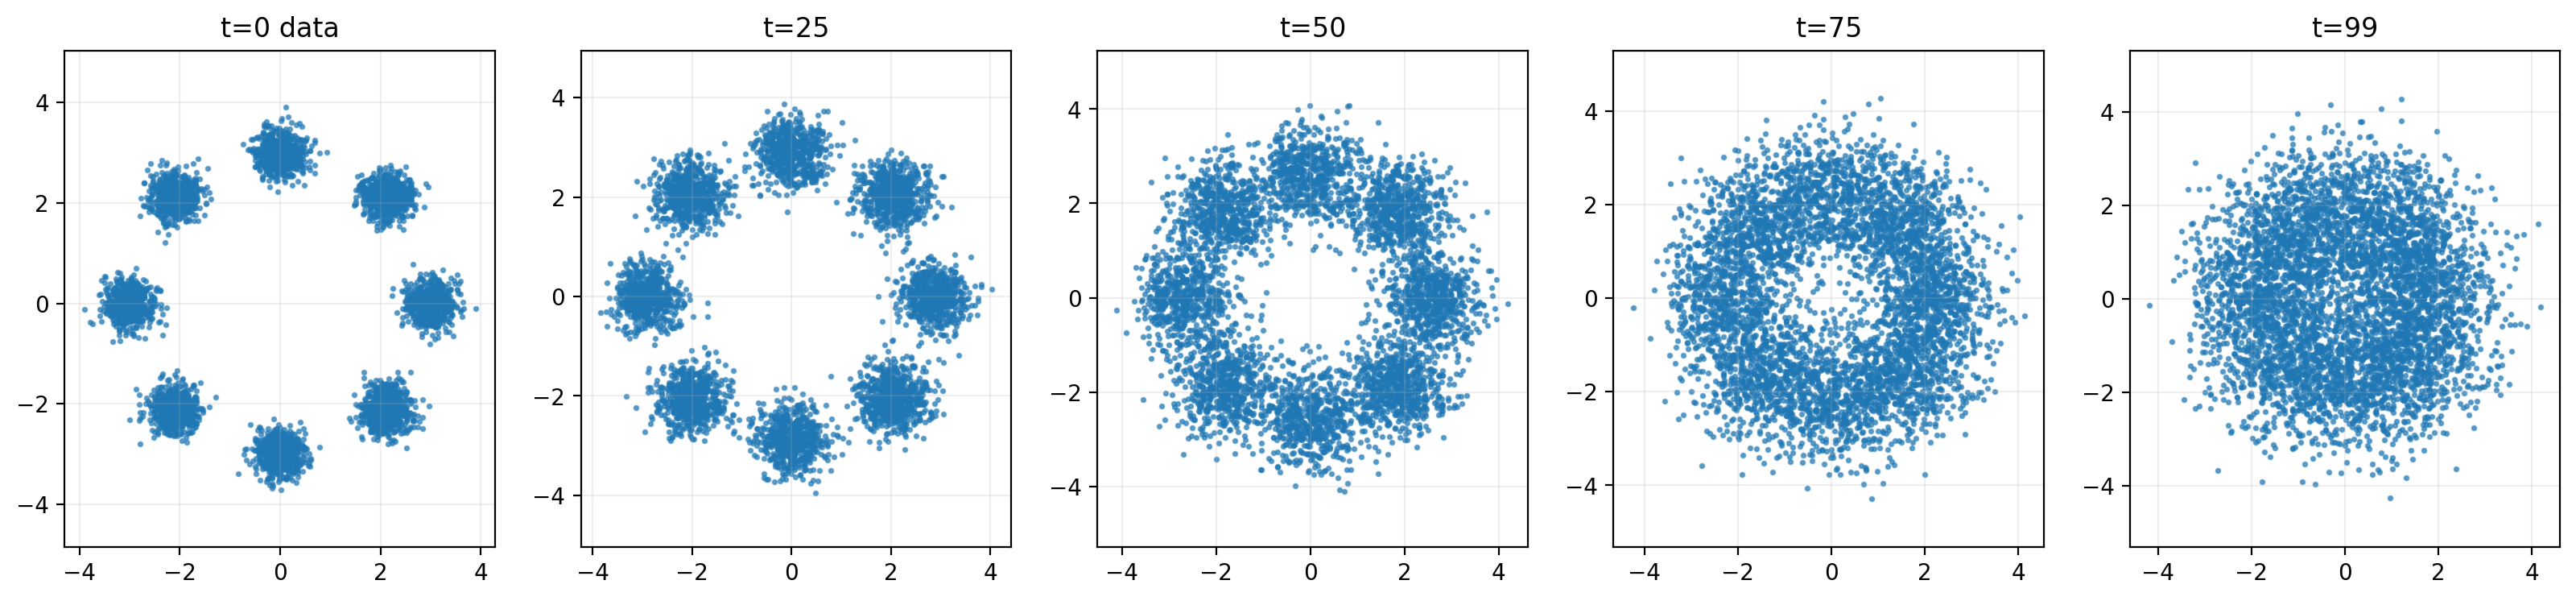
\includegraphics[width=\linewidth]{figures/stage3/forward_noising.png}
    \caption{前向加噪}
  \end{subfigure}
  \begin{subfigure}{0.32\linewidth}
    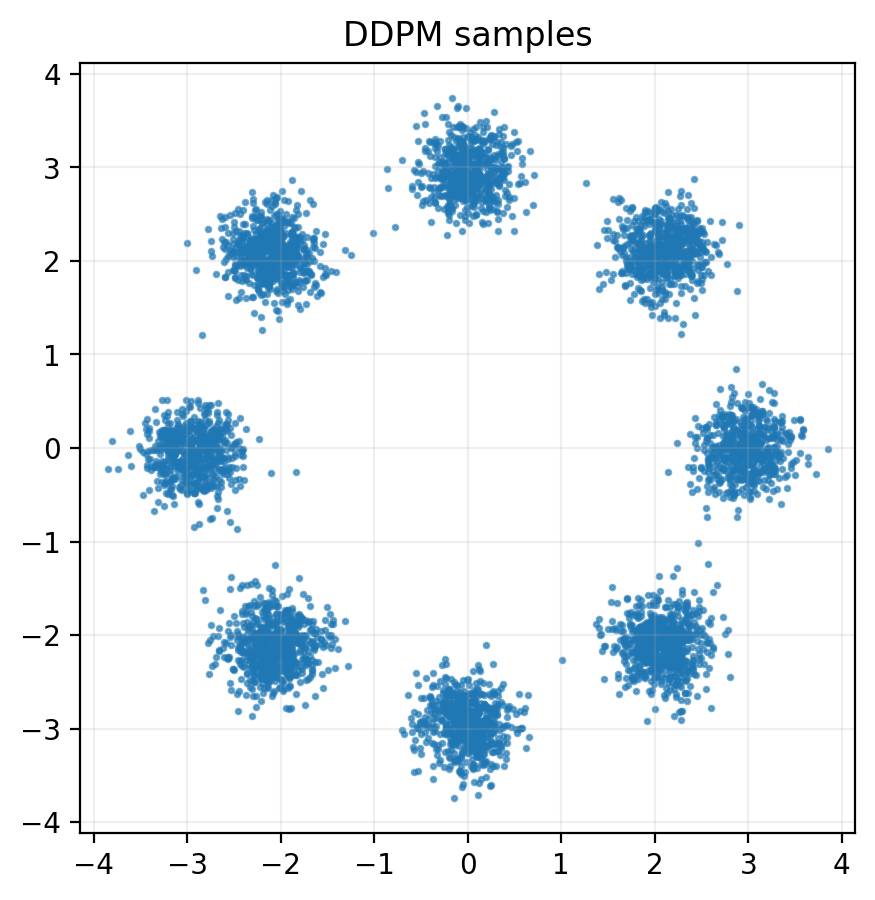
\includegraphics[width=\linewidth]{figures/stage3/ddpm_samples.png}
    \caption{DDPM 样本}
  \end{subfigure}
  \begin{subfigure}{0.32\linewidth}
    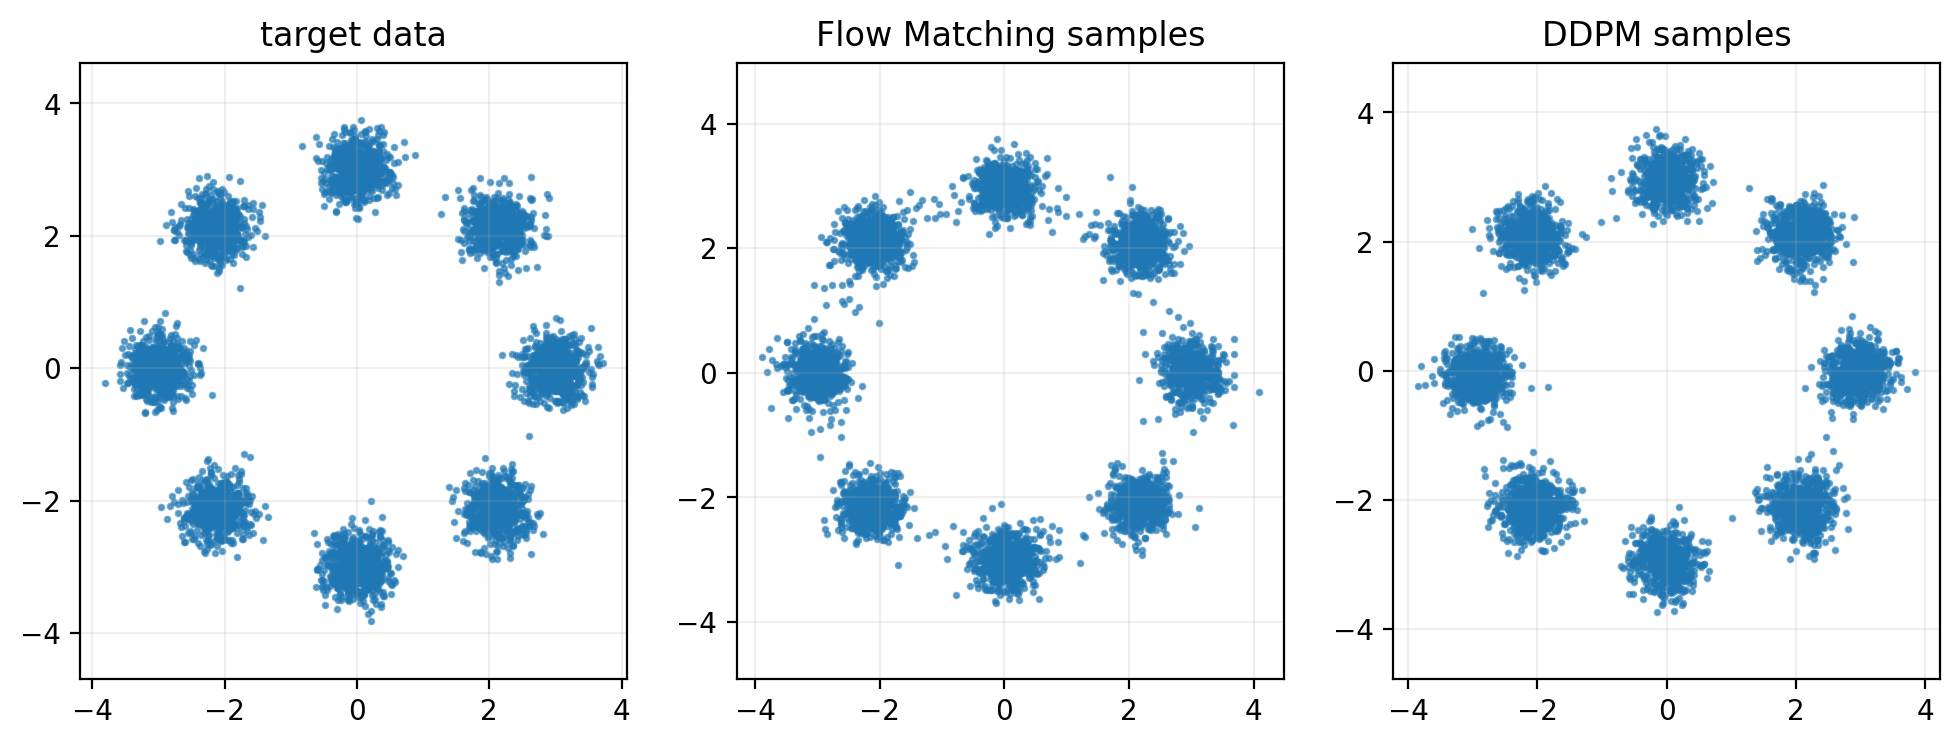
\includegraphics[width=\linewidth]{figures/stage3/fm_vs_ddpm.png}
    \caption{FM vs DDPM}
  \end{subfigure}
  \caption{DDPM 通过离散时间反向去噪生成样本，并与 Flow Matching 形成方法对照。}
\end{figure}

\paragraph{结果分析}
前向加噪图展示数据逐渐退化为噪声；采样轨迹展示反向去噪恢复结构。与 Flow Matching 相比，DDPM 的训练目标更成熟，后续在 CIFAR-10 上成为更强的定量 baseline。

\subsection{Lab 4：MNIST 条件扩散与 CFG}

\paragraph{理论基础}
Classifier-Free Guidance 在训练时随机丢弃类别标签，使模型同时学习条件与无条件预测；采样时使用
\[
  \epsilon_{\mathrm{cfg}}=\epsilon_{\mathrm{uncond}}+
  w(\epsilon_{\mathrm{cond}}-\epsilon_{\mathrm{uncond}}).
\]
更大的 $w$ 增强类别一致性，但可能牺牲多样性并引入伪影。

\paragraph{关键代码}
\begin{itemize}
  \item \code{src/time_embedding.py}：时间嵌入。
  \item \code{src/unet.py}：MNIST 条件 U-Net。
  \item \code{src/cfg_sampler.py}：CFG 采样。
  \item \code{labs/lab4/train_mnist_unet_cfg.py}、\code{labs/lab4/eval_cfg_scales.py}：训练与 scale 对比。
\end{itemize}

\begin{figure}[H]
  \centering
  \begin{subfigure}{0.48\linewidth}
    
\includegraphics[width=\linewidth]{figures/day4/class_cond_samples.png}
    \caption{类别条件生成}
  \end{subfigure}
  \begin{subfigure}{0.48\linewidth}
    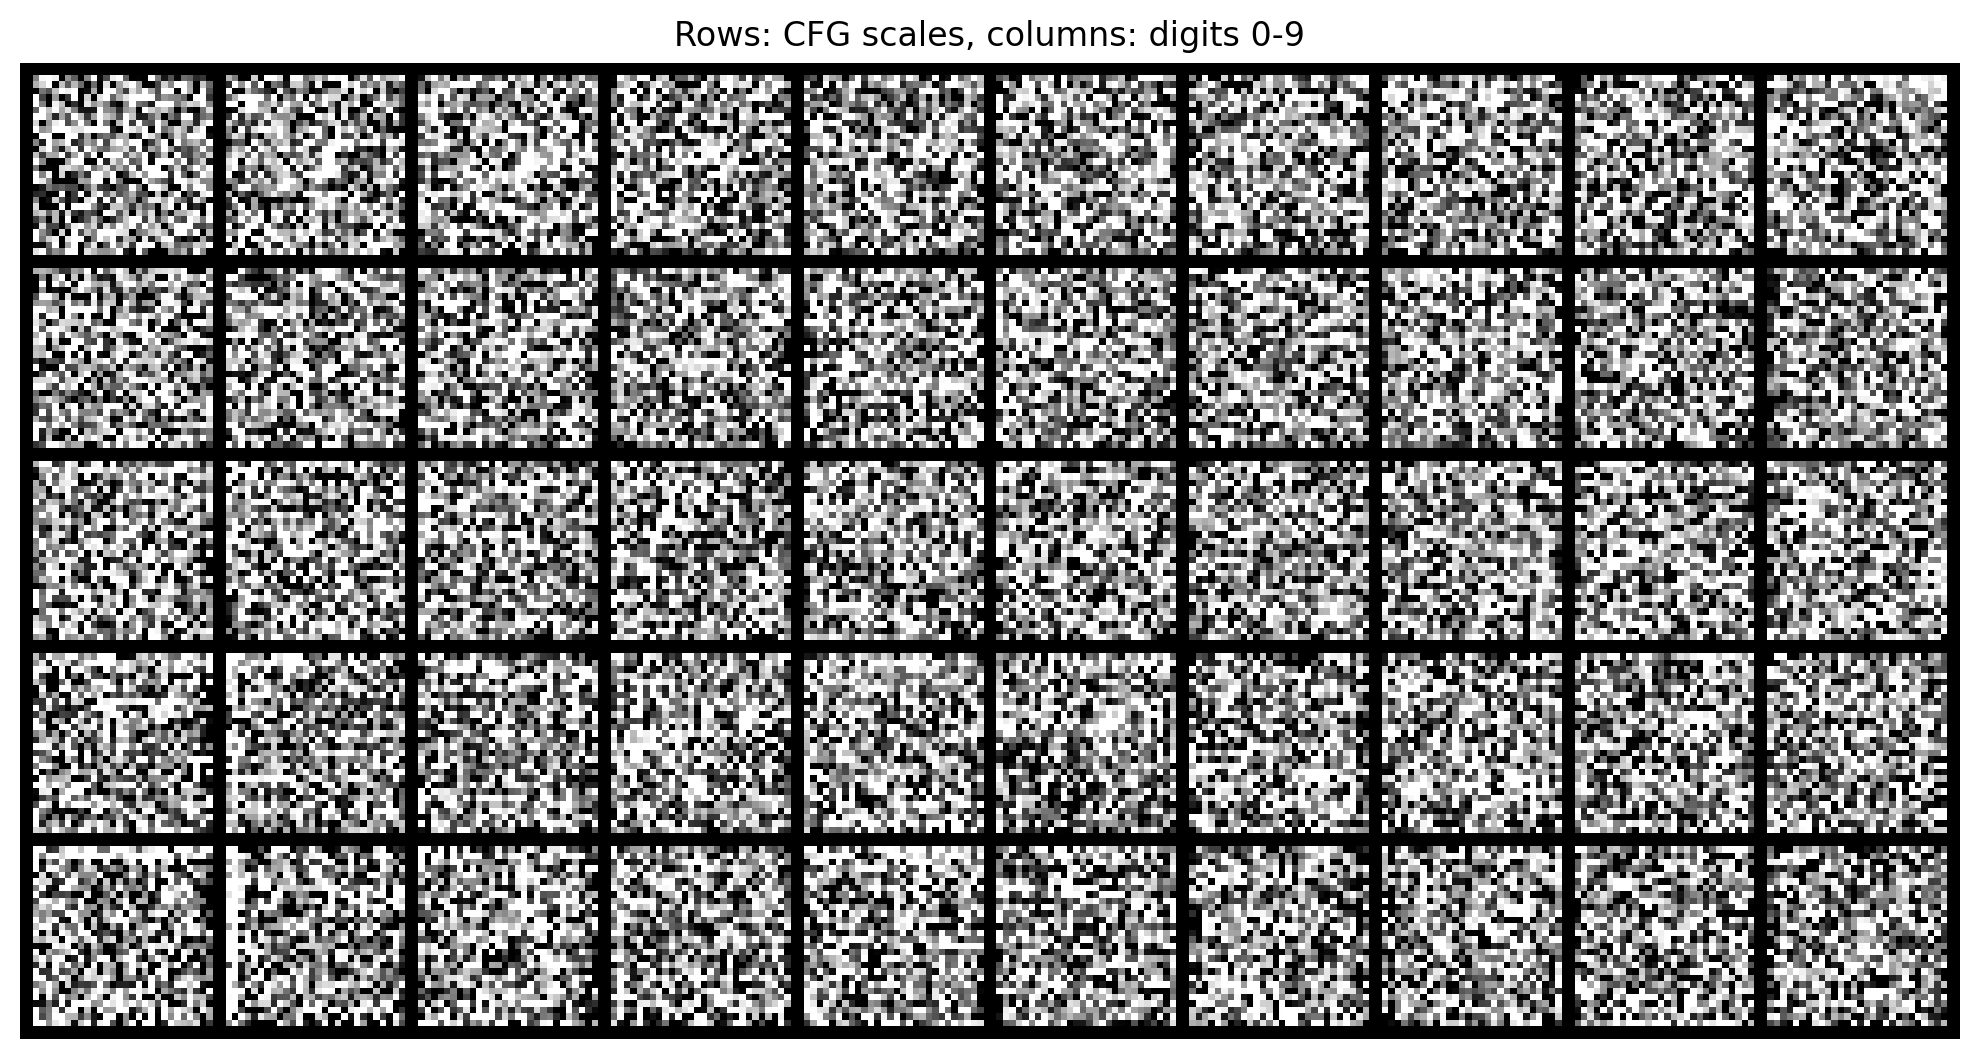
\includegraphics[width=\linewidth]{figures/day4/cfg_scale_comparison.png}
    \caption{CFG scale 对比}
  \end{subfigure}
  \caption{MNIST 条件扩散验证了类别控制与 guidance scale 的影响。}
\end{figure}

\paragraph{结果分析}
类别条件样本说明 U-Net 能根据数字标签控制生成结果。CFG scale 增大时数字类别更明确，但过高 scale 容易降低多样性。这个结论被迁移到 CIFAR-10 的 velocity guidance 与 DDPM/EDM CFG 实验。

\subsection{Lab 4.5：Mini-DiT 从零实现}

\paragraph{理论基础}
DiT 不是新的扩散目标，而是把 denoising network 从卷积 U-Net 换成 Transformer。图像被 patchify 成 token，经过 time/class conditioning 与 DiT block 后再 unpatchify 回图像空间。

\paragraph{关键代码}
\begin{itemize}
  \item \code{src/dit/patch_embed.py}：patchify 与 unpatchify。
  \item \code{src/dit/embeddings.py}：timestep 与 label embedding。
  \item \code{src/dit/dit_block.py}：AdaLN-Zero DiTBlock。
  \item \code{src/dit/model.py}：MiniDiT。
  \item \code{labs/lab_dit/train_mnist_dit.py}、\code{labs/lab_dit/compare_unet_dit.py}：训练与对比。
\end{itemize}

\begin{figure}[H]
  \centering
  \begin{subfigure}{0.32\linewidth}
    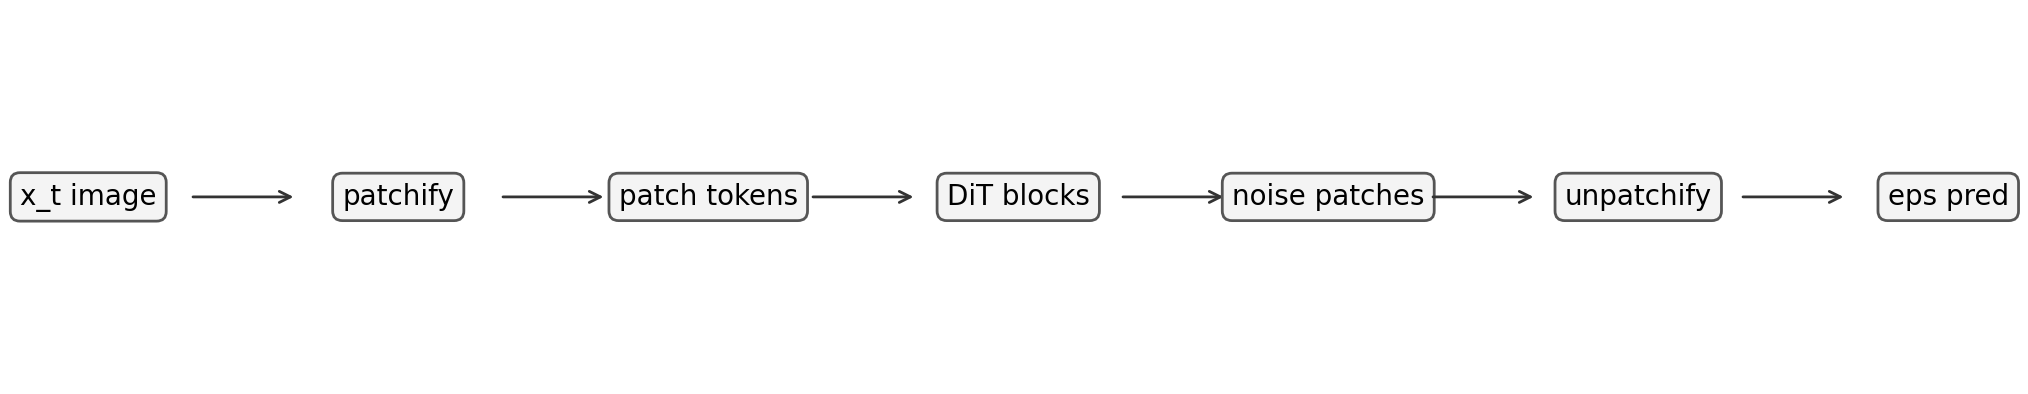
\includegraphics[width=\linewidth]{figures/dit/dit_architecture.png}
    \caption{DiT 架构}
  \end{subfigure}
  \begin{subfigure}{0.32\linewidth}
    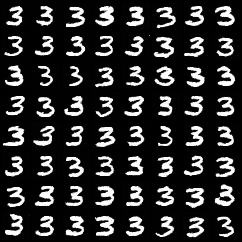
\includegraphics[width=\linewidth]{figures/dit/mnist_dit_samples.png}
    \caption{Mini-DiT 样本}
  \end{subfigure}
  \begin{subfigure}{0.32\linewidth}
    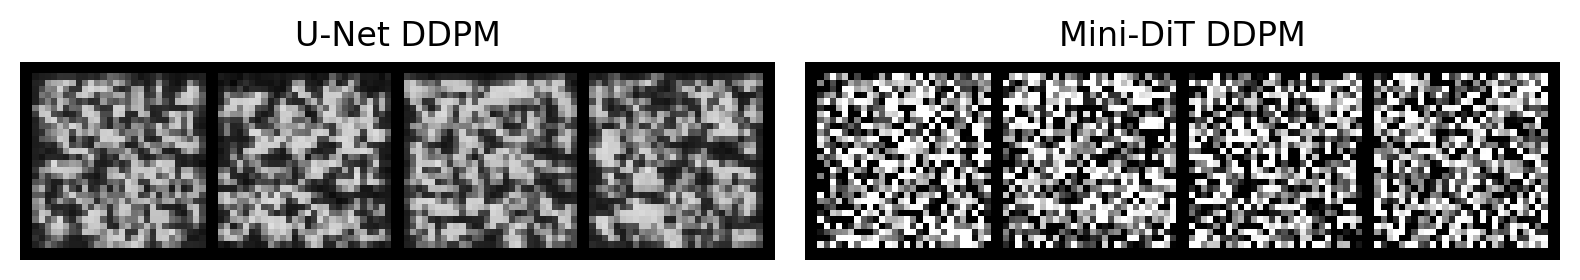
\includegraphics[width=\linewidth]{figures/dit/unet_vs_dit_samples.png}
    \caption{U-Net vs DiT}
  \end{subfigure}
  \caption{Mini-DiT Lab 完成了从 patch token 到图像预测的完整训练与采样闭环。}
\end{figure}

\paragraph{结果分析}
在 MNIST 小数据设置下，U-Net 依靠卷积归纳偏置更稳定；Mini-DiT 结构更通用，但需要更大数据和容量才能体现优势。因此展示项目没有在 U-Net baseline 尚不稳定时贸然扩展到 CIFAR-10 DiT。

\subsection{Lab 5：快速采样、离散扩散与统一理论}

\paragraph{理论基础}
Lab 5 总结连续扩散与离散扩散。连续模型关注 ODE/SDE、velocity 或 score；离散扩散通过 mask corruption 定义 token 状态转移，再训练反向 denoiser。

\paragraph{关键代码}
\begin{itemize}
  \item \code{src/discrete_diffusion.py}：mask corruption 与离散转移。
  \item \code{src/discrete_denoiser.py}：toy sequence denoiser。
  \item \code{labs/lab5/02_run_mask_corruption.py}：前向 mask corruption。
  \item \code{labs/lab5/03_train_discrete_denoiser.py}、\code{labs/lab5/04_sample_discrete_denoiser.py}：离散 denoiser 训练与采样。
  \item \code{src/theory_plotting.py}、\code{labs/lab5/05_make_stage5_figures.py}：统一理论图。
\end{itemize}

\begin{figure}[H]
  \centering
  \begin{subfigure}{0.32\linewidth}
    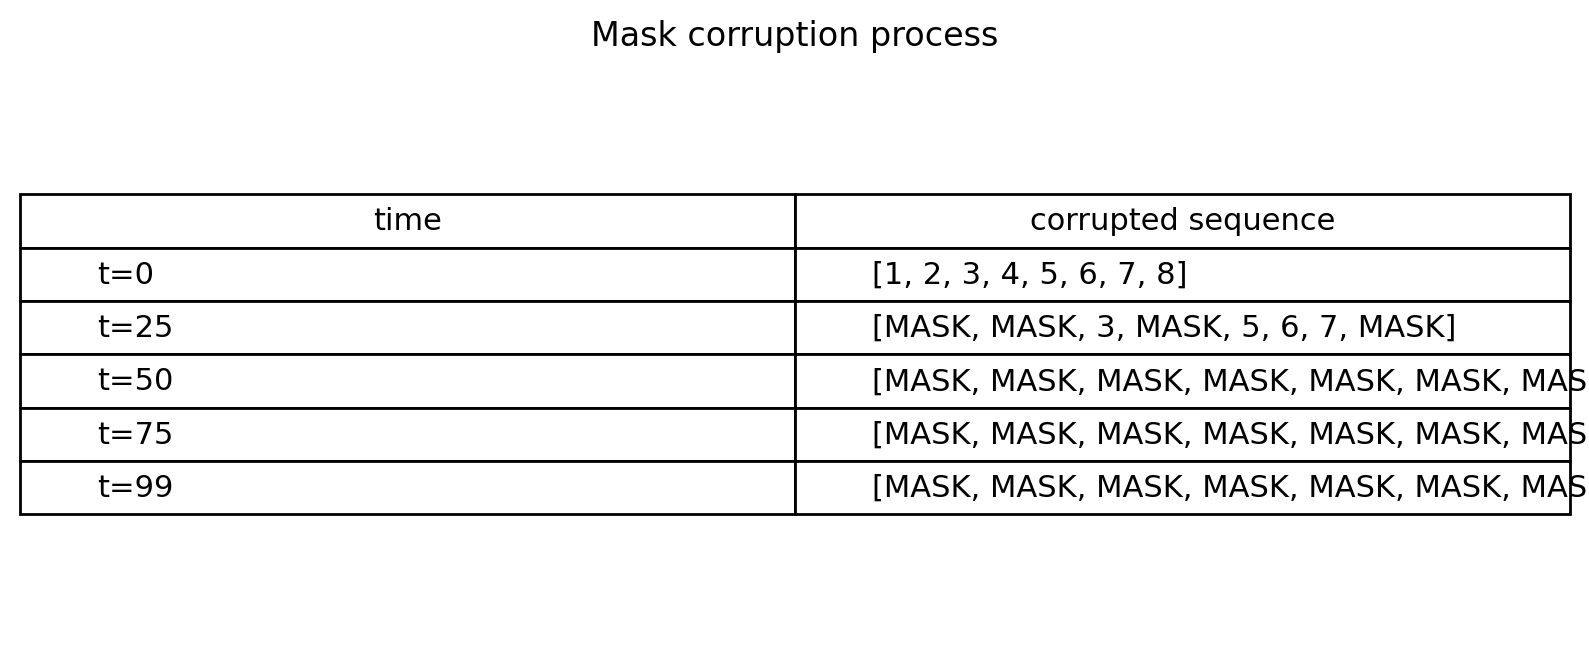
\includegraphics[width=\linewidth]{figures/day5/mask_corruption_process.png}
    \caption{Mask corruption}
  \end{subfigure}
  \begin{subfigure}{0.32\linewidth}
    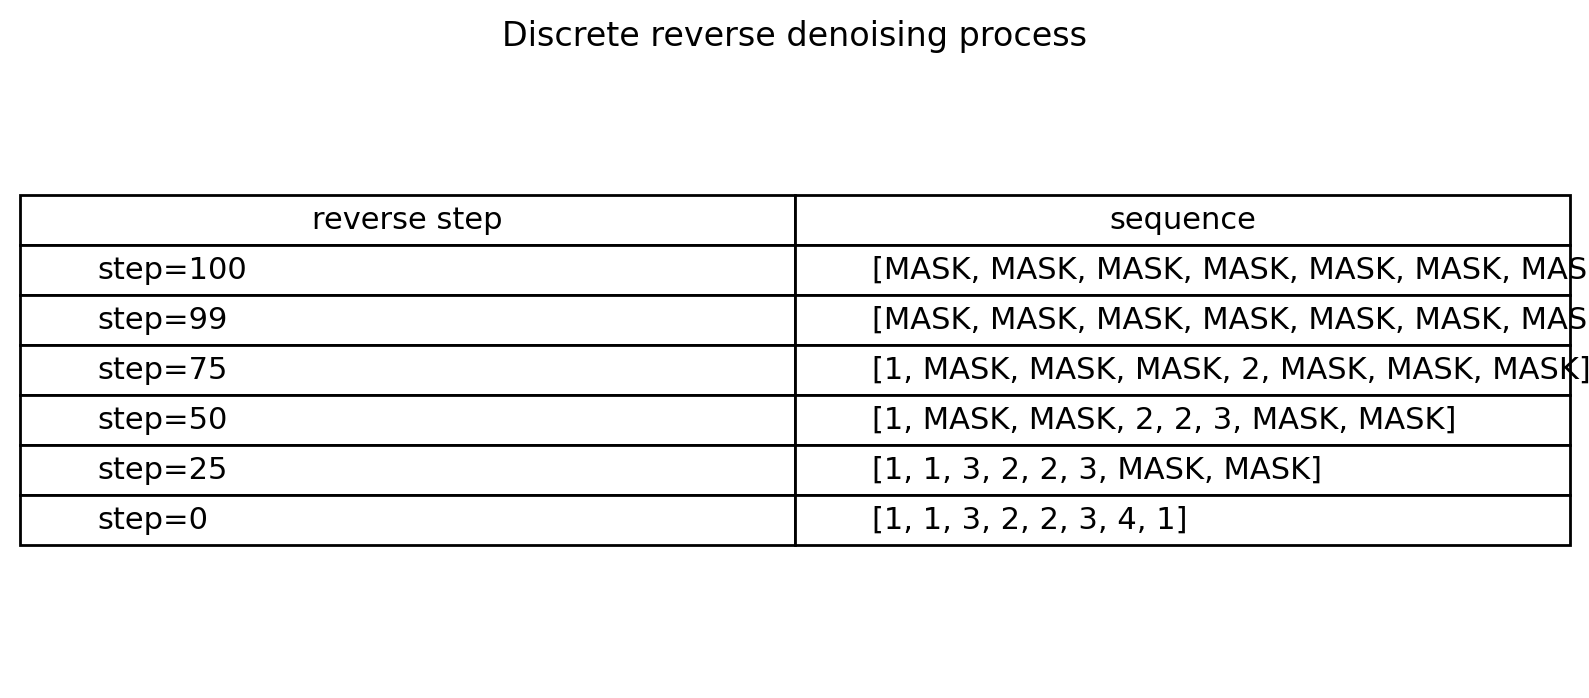
\includegraphics[width=\linewidth]{figures/day5/discrete_reverse_process.png}
    \caption{离散反向过程}
  \end{subfigure}
  \begin{subfigure}{0.32\linewidth}
    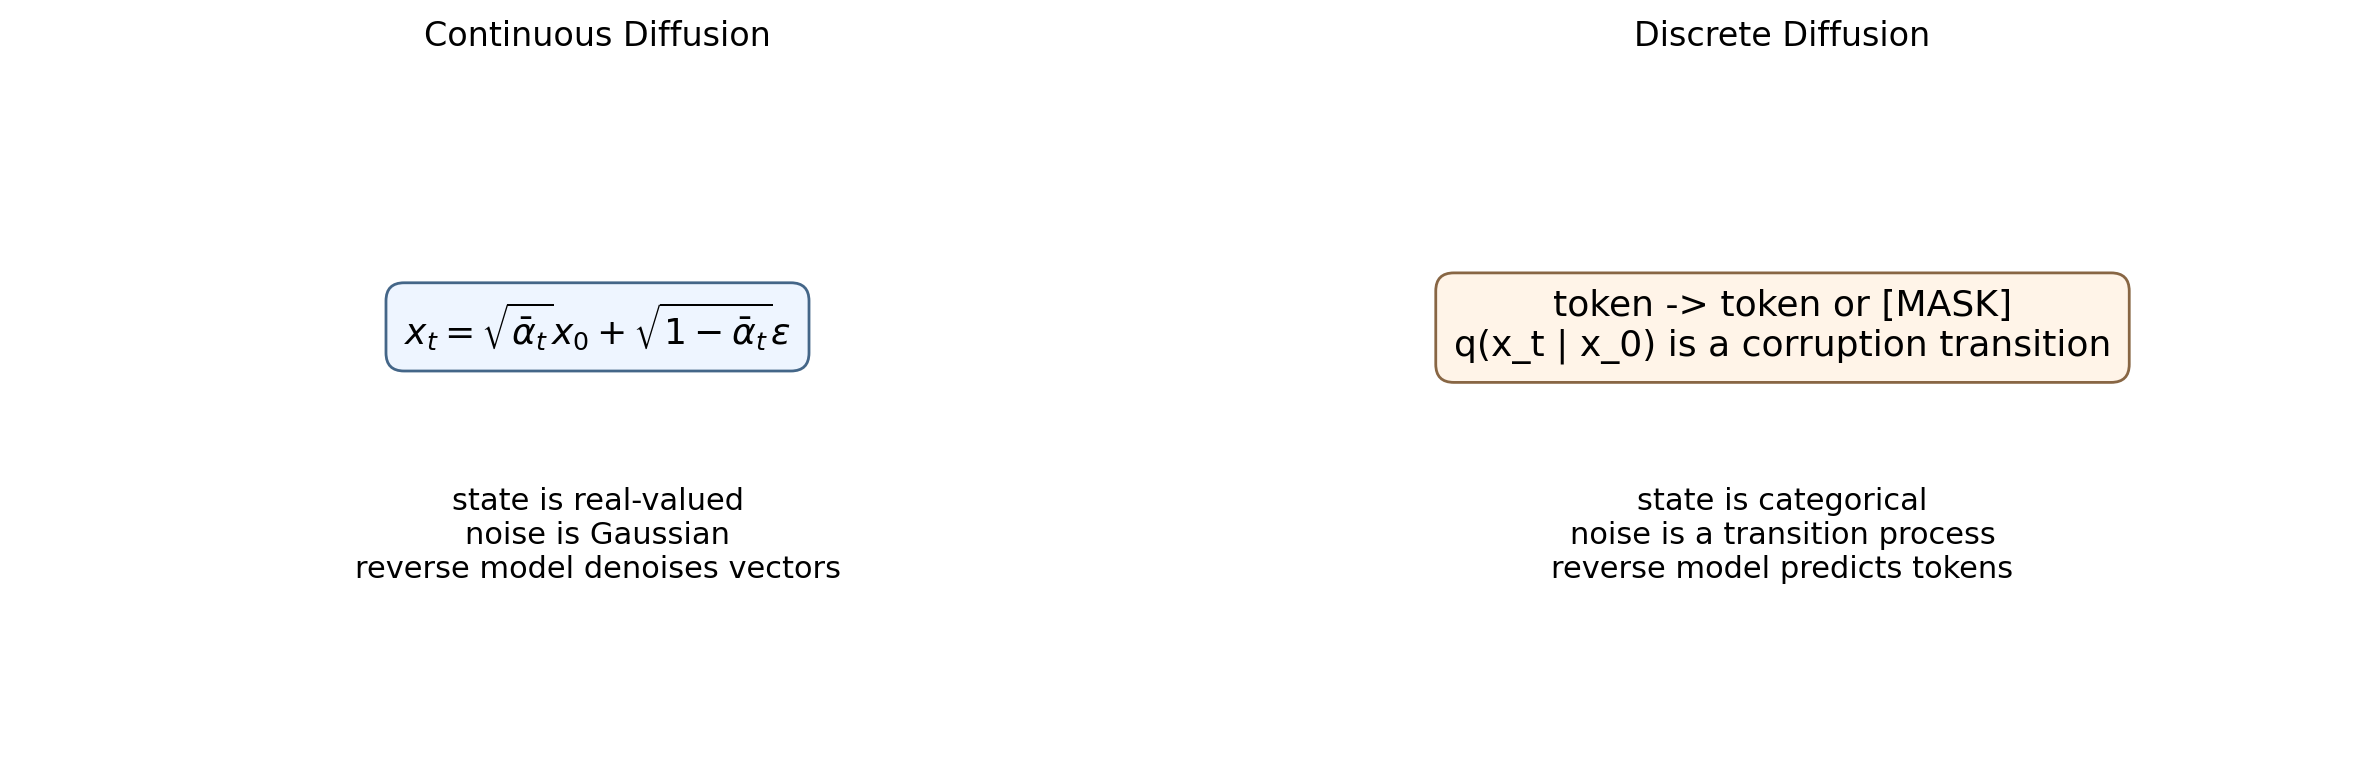
\includegraphics[width=\linewidth]{figures/day5/continuous_vs_discrete_diffusion.png}
    \caption{连续 vs 离散}
  \end{subfigure}
  \caption{Stage 5 将连续生成模型和离散扩散模型放入统一总结中。}
\end{figure}

\paragraph{结果分析}
mask corruption 图显示 token 随 $t$ 增大逐步被 mask；reverse process 展示 denoiser 如何从全 mask 恢复训练模式。统一理论图说明：DDPM、Flow Matching、Rectified Flow 和离散扩散的差异主要在路径、状态空间和预测函数。

\section{第二部分：展示项目阶段总结}

\subsection{阶段 A：CIFAR-10 U-Net Rectified Flow Baseline}

\paragraph{方法与改进}
展示项目首先落地类别条件 Rectified Flow。相比二维 toy Lab，本阶段把 $x_t=(1-t)x_0+t x_1$ 扩展到 CIFAR-10 图像，并使用 U-Net 预测 velocity field。类别标签通过 embedding 注入网络，采样使用 Euler/Heun ODE solver。

\paragraph{关键代码与配置}
\begin{itemize}
  \item \code{src/cifar10_dataset.py}：CIFAR-10 dataloader，归一化到 $[-1,1]$。
  \item \code{src/image_flow_matching.py}：图像 Rectified Flow tuple 与 loss。
  \item \code{src/image_unet.py}：类别条件 U-Net velocity network。
  \item \code{labs/lab_cifar_flow/train_cifar10_unet_fm.py}：训练入口。
  \item \code{configs/cifar10_unet_fm.yaml}：baseline 配置。
\end{itemize}

\begin{figure}[H]
  \centering
  \begin{subfigure}{0.32\linewidth}
    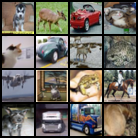
\includegraphics[width=\linewidth]{figures/cifar_flow/debug/debug_real_images.png}
    \caption{真实图像}
  \end{subfigure}
  \begin{subfigure}{0.32\linewidth}
    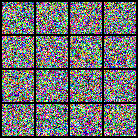
\includegraphics[width=\linewidth]{figures/cifar_flow/debug/debug_noise_images.png}
    \caption{高斯噪声}
  \end{subfigure}
  \begin{subfigure}{0.32\linewidth}
    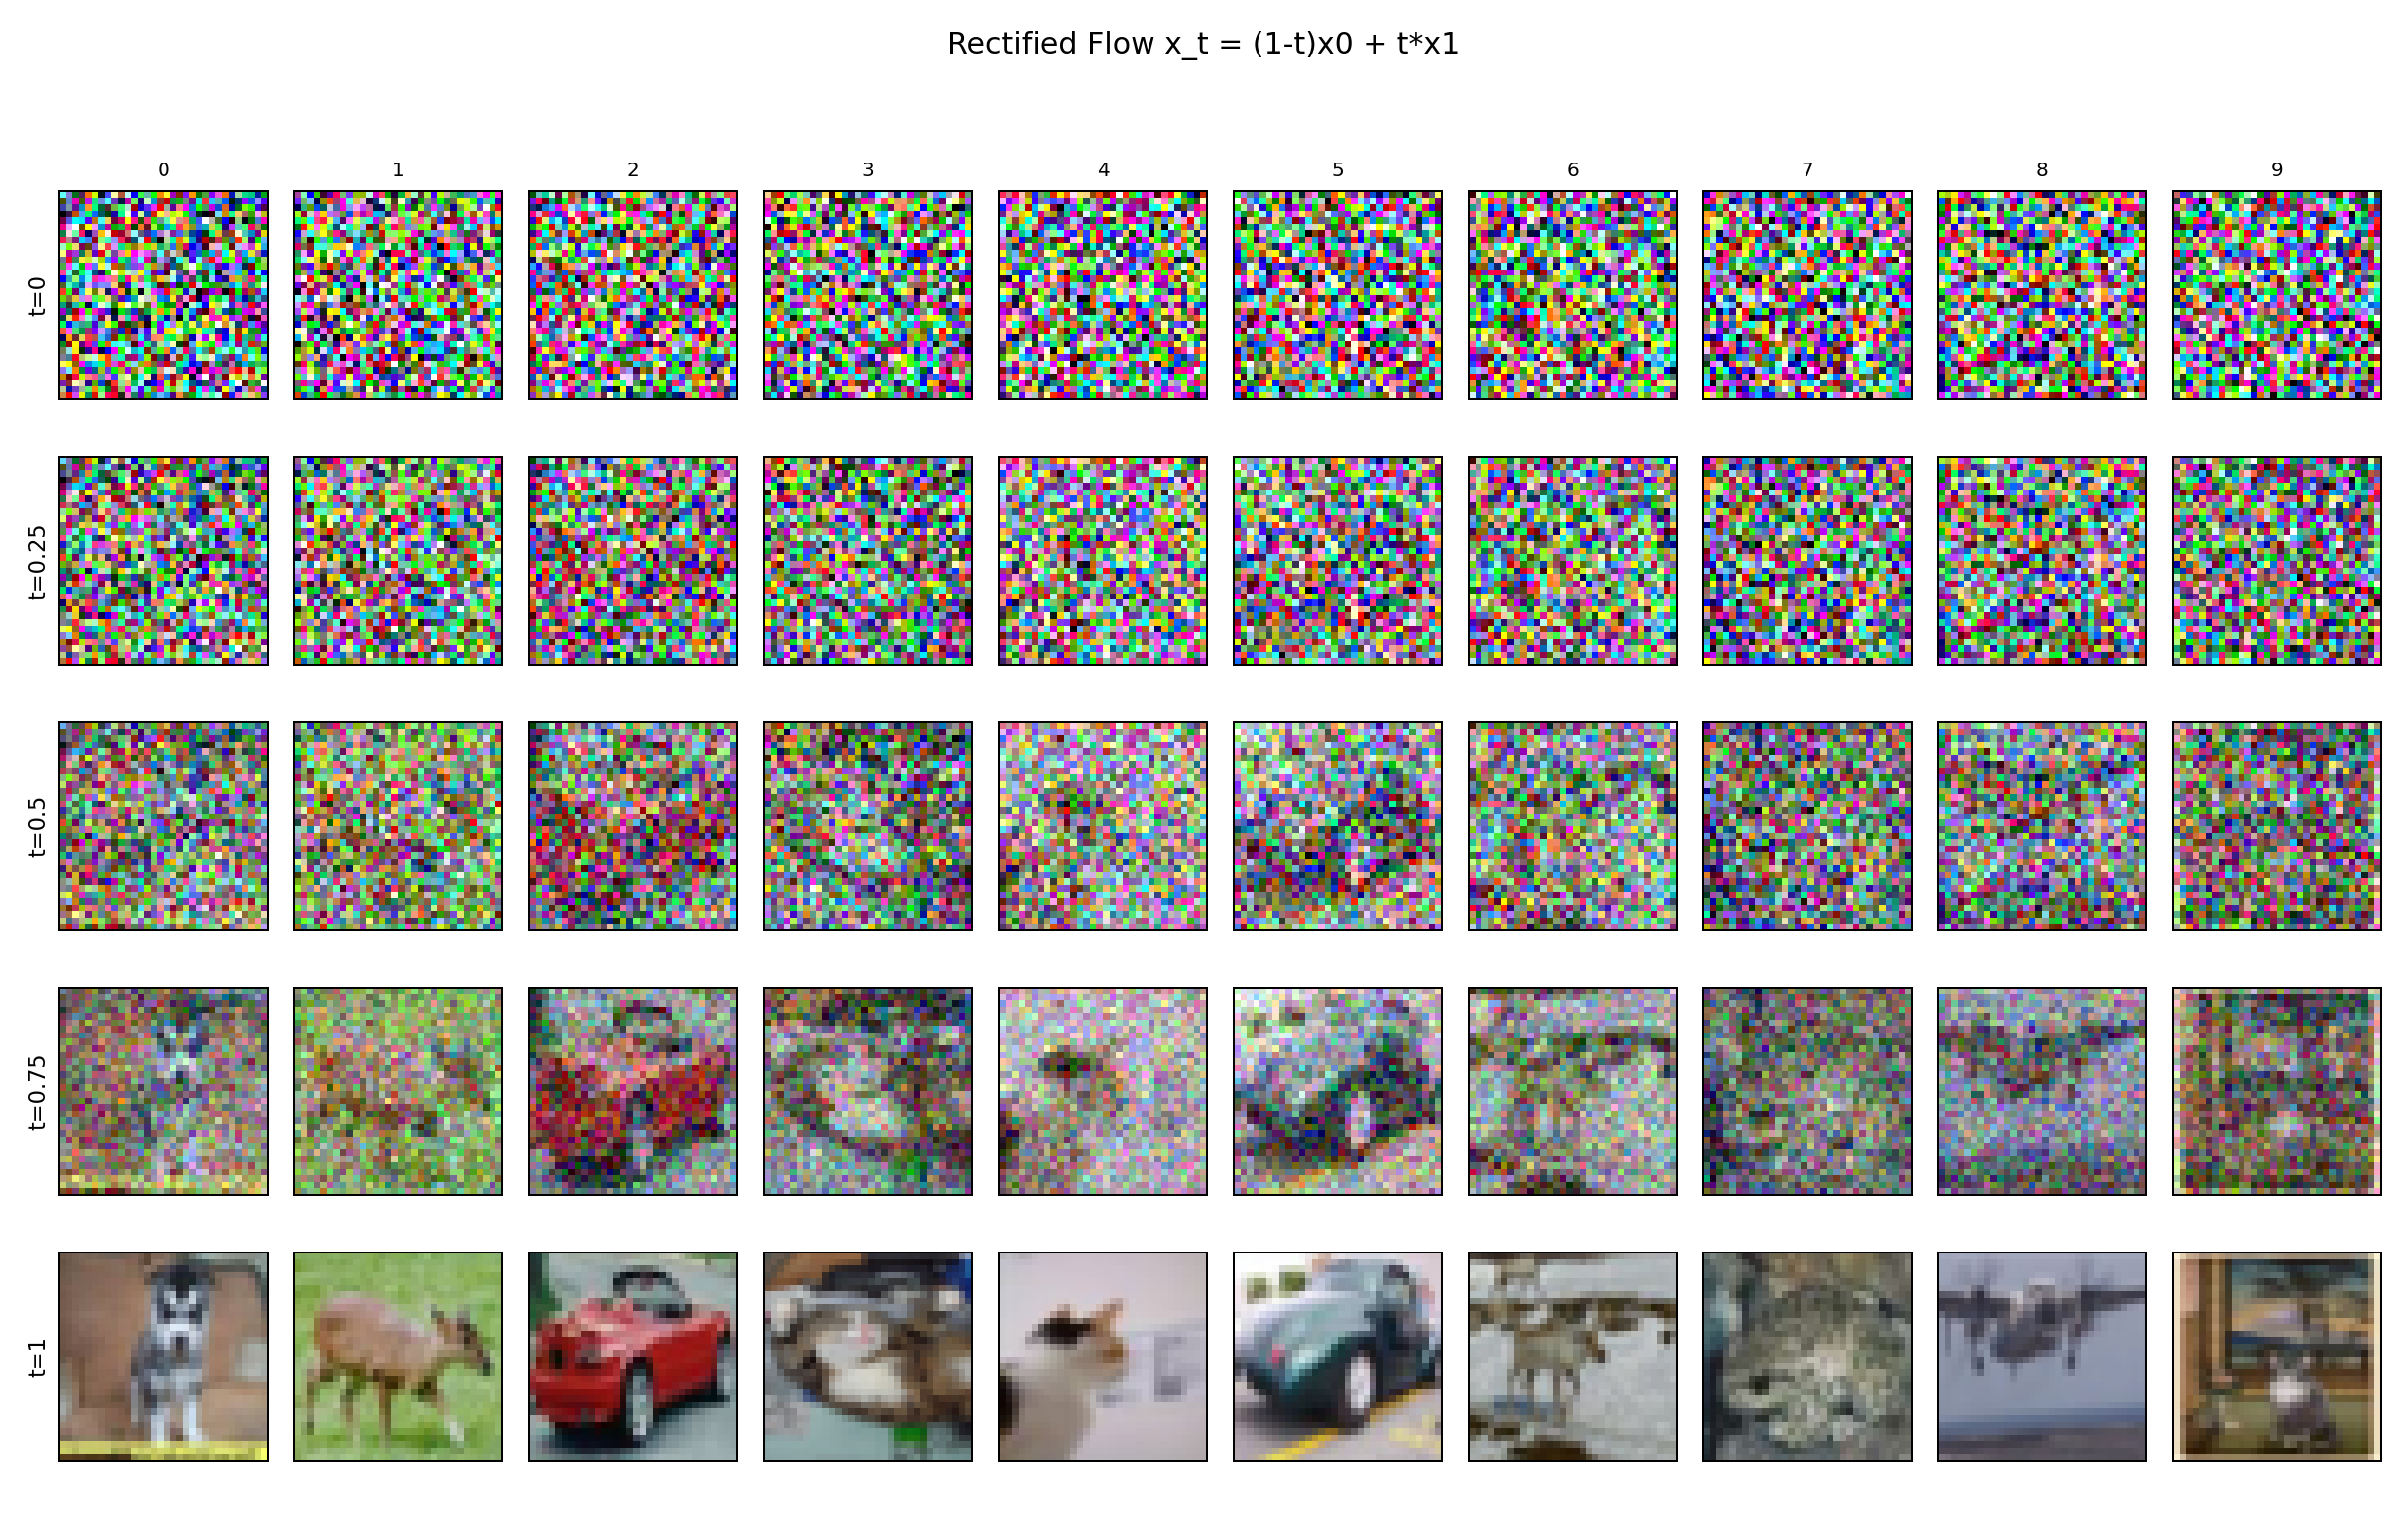
\includegraphics[width=\linewidth]{figures/cifar_flow/debug/debug_xt_interpolation.png}
    \caption{$x_t$ 插值}
  \end{subfigure}
  \caption{进入长训前先检查数据、噪声、插值与保存逻辑，排除 pipeline bug。}
\end{figure}

\begin{figure}[H]
  \centering
  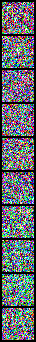
\includegraphics[width=0.86\linewidth]{figures/cifar_flow/class_conditional_samples.png}
  \caption{第一版 CIFAR-10 Rectified Flow 生成结果：已脱离纯噪声，但结构较糊。}
\end{figure}

\paragraph{困难与解决}
主要困难是样本偏模糊，类别结构弱。我们先不急于扩展 Mini-DiT，而是做 debug 图确认真实图、噪声、插值和反归一化正确，避免把代码 bug 误判为模型问题。

\paragraph{消融与结论}
第一阶段完成了训练闭环，但视觉质量不足。结论是：Rectified Flow baseline 可用于研究速度场和 ODE 采样，但还需要质量升级。

\subsection{阶段 B：NFE、Solver 与 Guidance 消融}

\paragraph{方法与改进}
在同一个 U-Net Rectified Flow checkpoint 上，系统比较 NFE、Euler/Heun solver、CFG-like velocity guidance 和 runtime/memory。相比阶段 A，这一阶段从“能出图”升级为“能分析采样过程”。

\paragraph{实验结果}
\begin{figure}[H]
  \centering
  \begin{subfigure}{0.48\linewidth}
    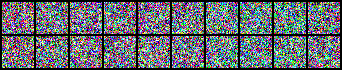
\includegraphics[width=\linewidth]{figures/cifar_flow/nfe_ablation_unet.png}
    \caption{NFE 消融}
  \end{subfigure}
  \begin{subfigure}{0.48\linewidth}
    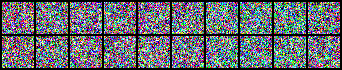
\includegraphics[width=\linewidth]{figures/cifar_flow/solver_ablation_unet.png}
    \caption{Euler vs Heun}
  \end{subfigure}
  \begin{subfigure}{0.48\linewidth}
    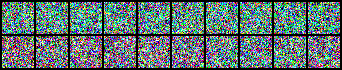
\includegraphics[width=\linewidth]{figures/cifar_flow/guidance_ablation_unet.png}
    \caption{Guidance scale}
  \end{subfigure}
  \begin{subfigure}{0.48\linewidth}
    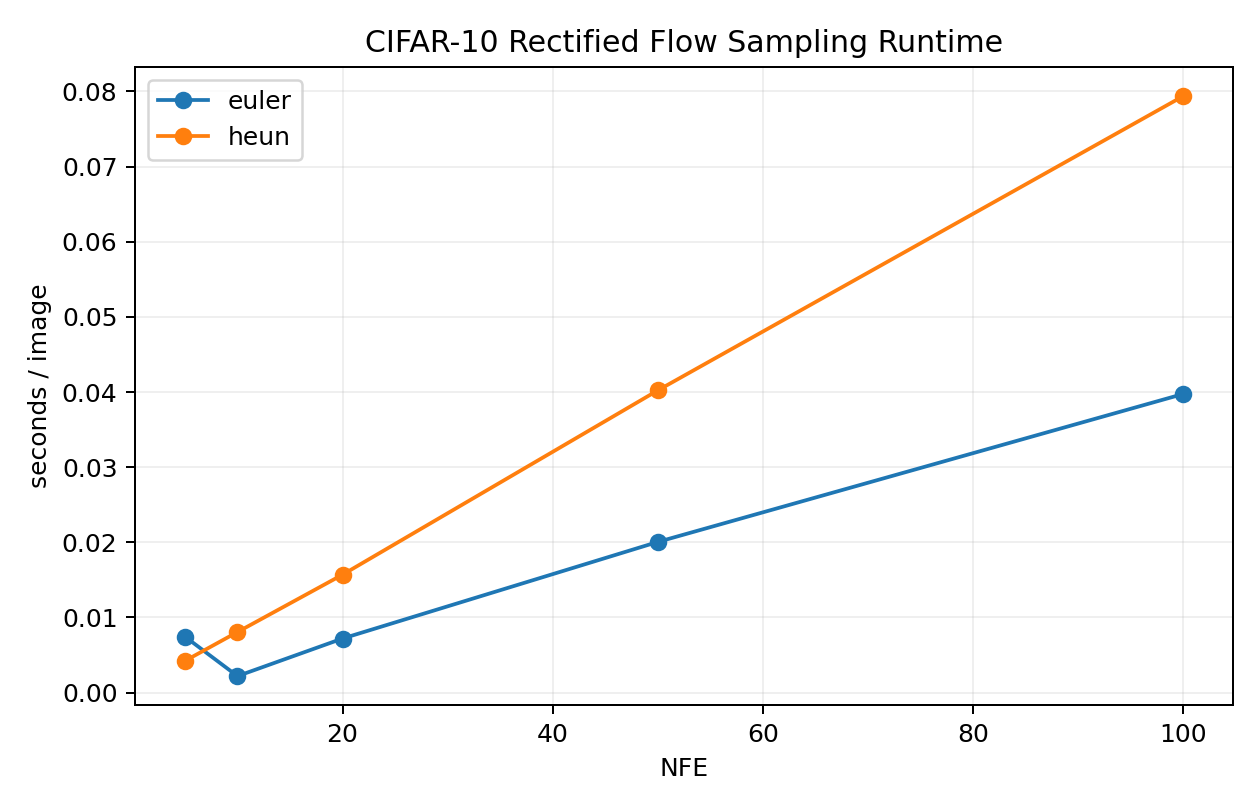
\includegraphics[width=\linewidth]{figures/cifar_flow/runtime_vs_nfe.png}
    \caption{Runtime vs NFE}
  \end{subfigure}
  \caption{Phase 2 采样分析：质量、速度和类别控制之间存在明确 trade-off。}
\end{figure}

\paragraph{困难与解决}
低 NFE 容易产生不完整结构，高 guidance scale 可能放大伪影。解决方式是把低 NFE 作为速度分析，而不是质量判断；质量评估统一采用更高 NFE 和 Heun。

\paragraph{消融结论}
NFE=50/100 通常比 NFE=5 稳定；Heun 在低 NFE 下更平滑但计算更慢；guidance 能增强类别方向，但过强 guidance 会降低自然度。

\subsection{阶段 C：Rectified Flow 质量升级}

\paragraph{方法与改进}
针对“图像仍然很糊”的问题，阶段 C 对 U-Net Rectified Flow 做质量升级：EMA、attention U-Net、更长训练、beta time sampling、data-end loss weighting、OT/minibatch pairing 和更大容量配置。相比阶段 B，这一阶段不再横向增加 sampler，而是集中提升生成能力。

\paragraph{实验结果}
\begin{figure}[H]
  \centering
  \begin{subfigure}{0.48\linewidth}
    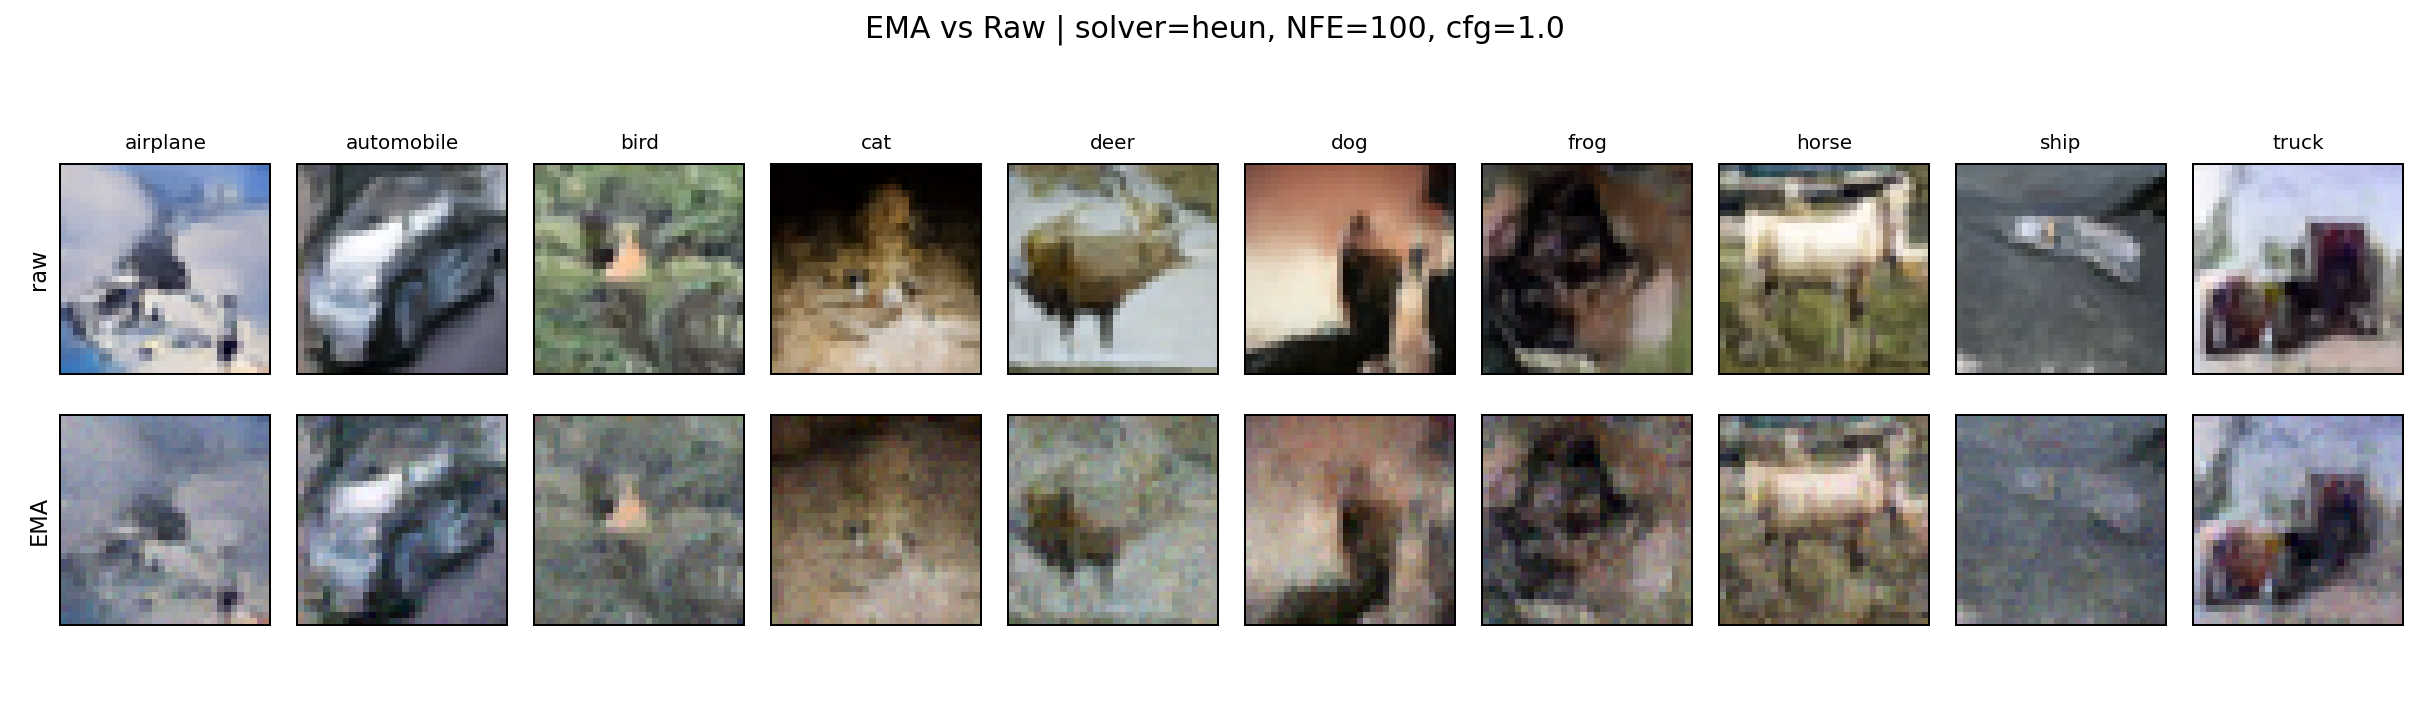
\includegraphics[width=\linewidth]{figures/cifar_flow/ema_vs_raw_100ep.png}
    \caption{EMA vs raw}
  \end{subfigure}
  \begin{subfigure}{0.48\linewidth}
    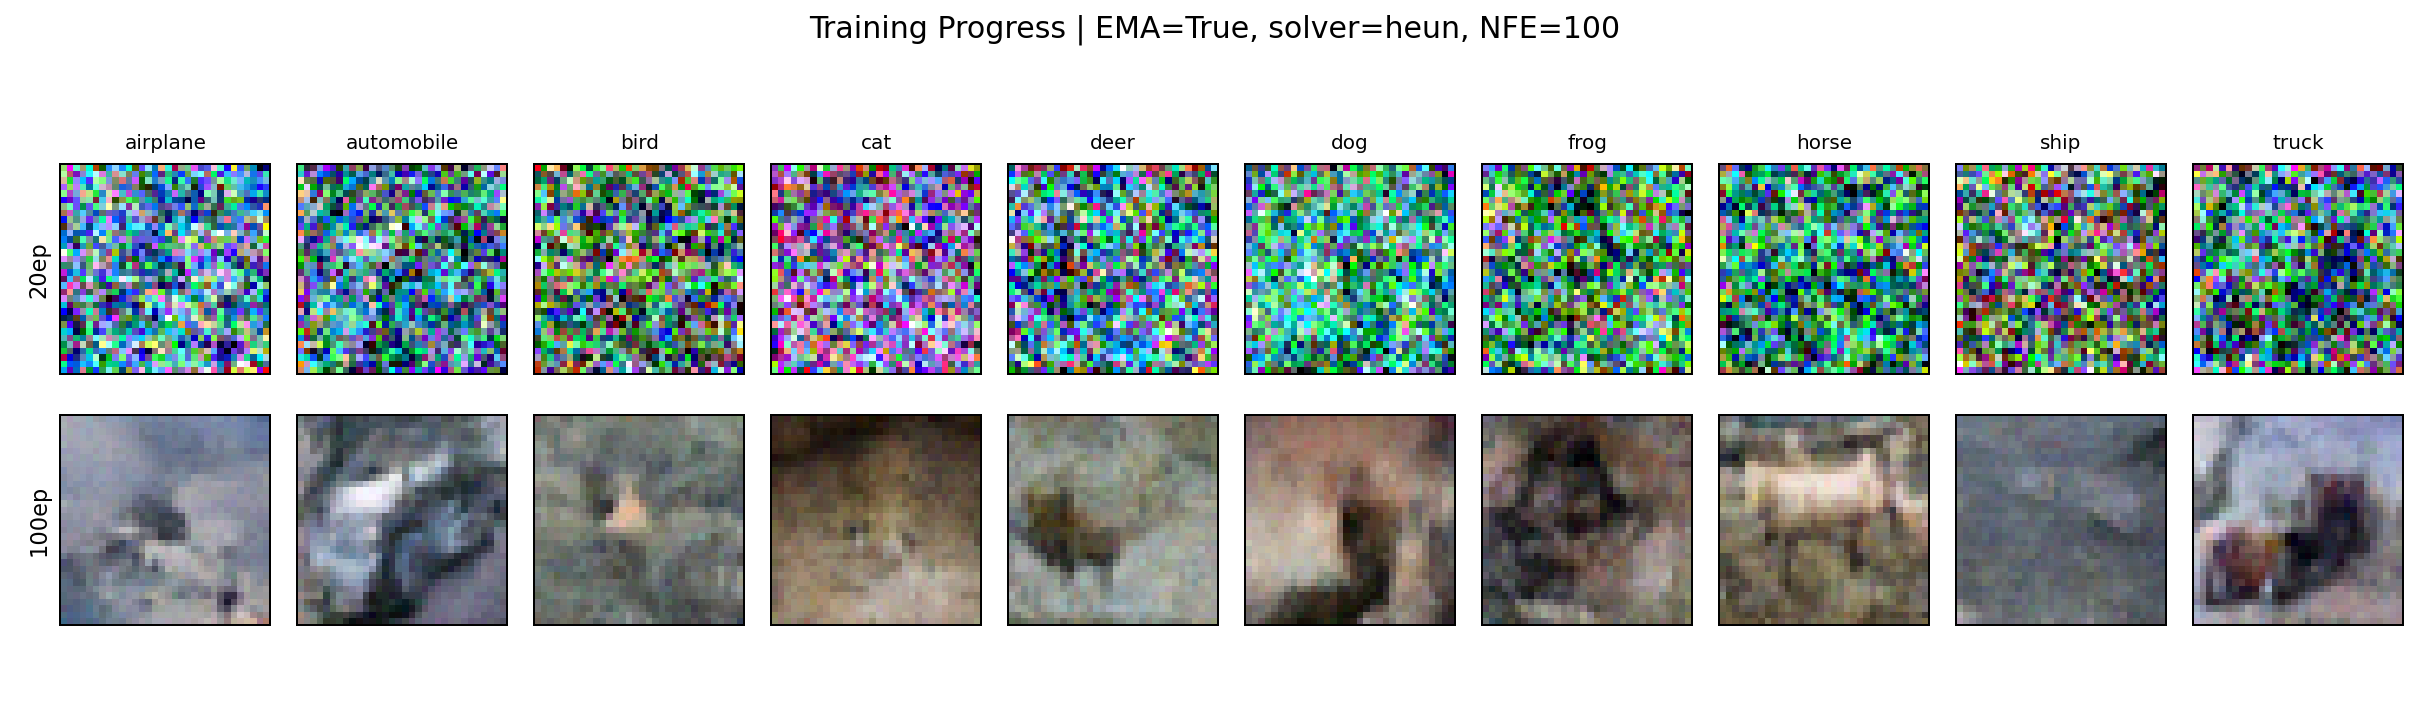
\includegraphics[width=\linewidth]{figures/cifar_flow/training_progress_20ep_vs_100ep.png}
    \caption{20ep vs 100ep}
  \end{subfigure}
  \begin{subfigure}{0.48\linewidth}
    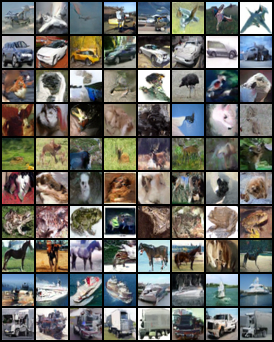
\includegraphics[width=\linewidth]{figures/cifar_flow/class_conditional_samples_v2_300ep.png}
    \caption{Attention U-Net 300ep}
  \end{subfigure}
  \begin{subfigure}{0.48\linewidth}
    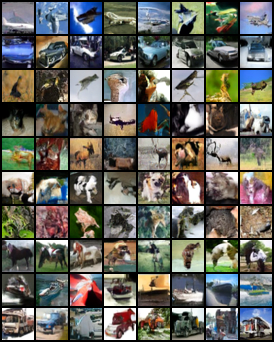
\includegraphics[width=\linewidth]{figures/cifar_flow/class_conditional_samples_v2_beta41_dataend2_300ep.png}
    \caption{Time sampling + weighting}
  \end{subfigure}
  \caption{Rectified Flow 质量升级带来可见改善，但仍未达到最终展示质量。}
\end{figure}

\paragraph{困难与解决}
训练 loss 已收敛但图仍糊，说明 MSE velocity loss 与视觉质量并不完全一致。我们通过 EMA 平滑权重、attention 增强全局建模、data-end weighting 强化靠近数据端的训练信号，并保留每次实验配置以便复现。

\paragraph{消融结论}
100 epochs 明显优于 20 epochs，300 epochs 继续改善但边际收益下降；EMA 提升稳定性；time sampling 和 loss weighting 略有收益；但仅靠 Rectified Flow 继续堆 epoch 不是最优路线。因此项目转向更成熟的 DDPM/DDIM baseline。

\subsection{阶段 D：DDPM/DDIM 强 Baseline}

\paragraph{方法与改进}
为了获得最终效果，阶段 D 使用 DDPM 训练目标、cosine schedule、v-prediction 和 DDIM 采样。相比 Rectified Flow 分支，DDPM/DDIM 的训练和采样更成熟，适合作为 CIFAR-10 定量主结果。

\paragraph{关键代码}
\begin{itemize}
  \item \code{labs/lab_cifar_flow/train_cifar10_ddpm_unet.py}
  \item \code{labs/lab_cifar_flow/sample_cifar10_ddpm.py}
  \item \code{labs/lab_cifar_flow/eval_cifar10_ddpm_metrics.py}
  \item \code{configs/cifar10_unet_ddpm_cosine_vpred_500ep.yaml}
  \item \code{configs/cifar10_final_showcase_cosine_vpred_upscaled.yaml}
\end{itemize}

\begin{figure}[H]
  \centering
  \begin{subfigure}{0.58\linewidth}
    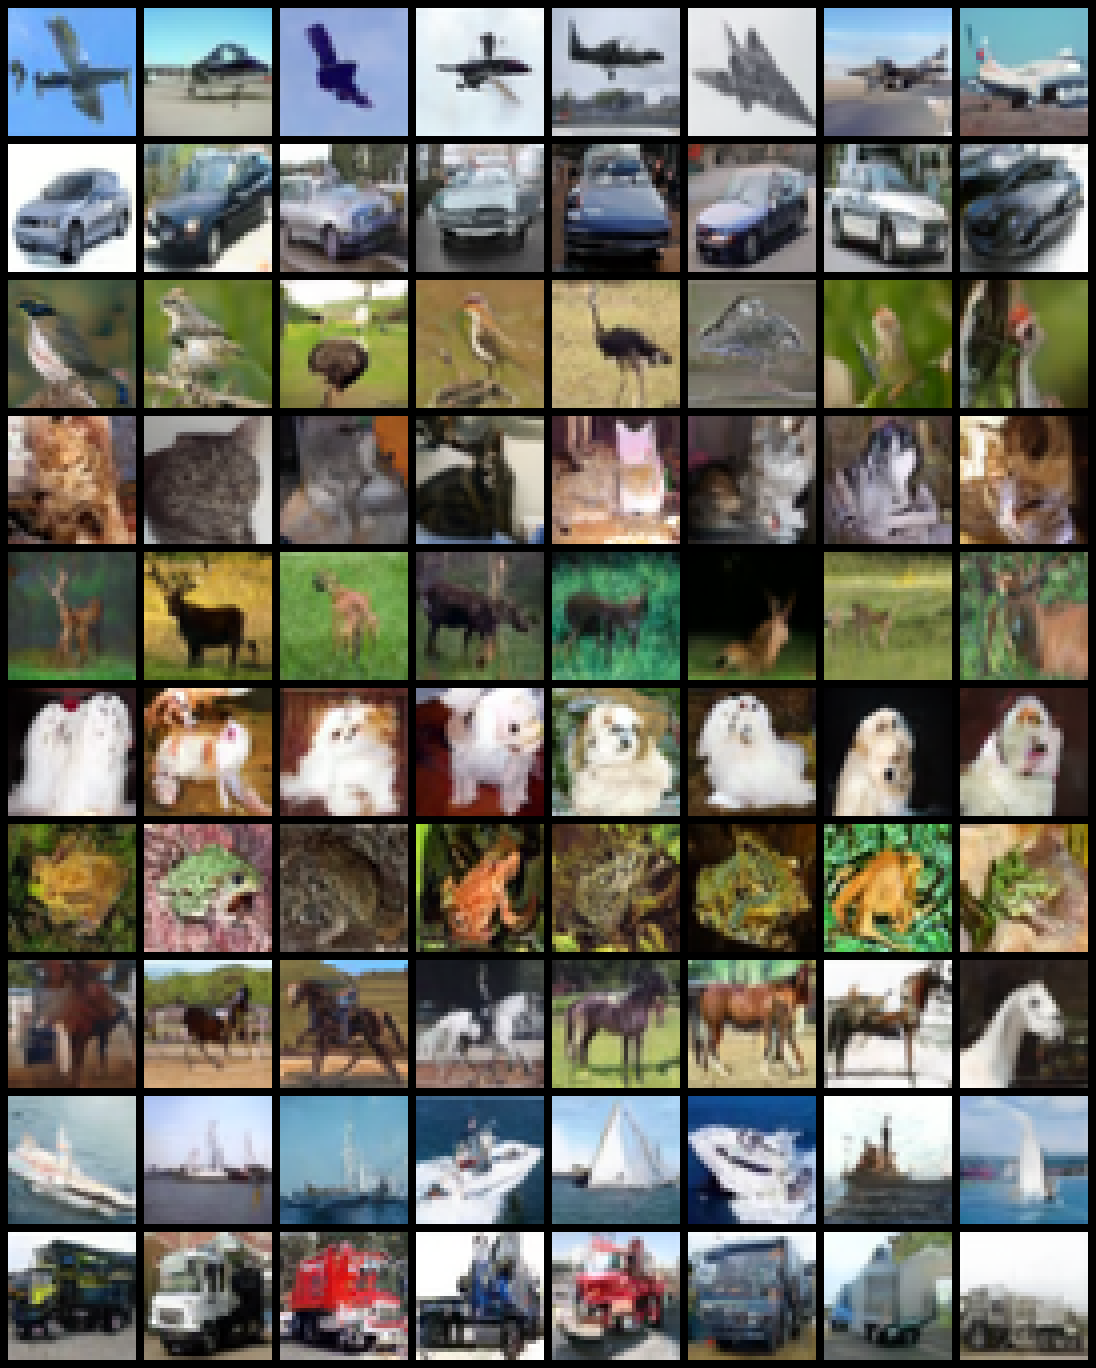
\includegraphics[width=\linewidth]{figures/cifar_flow/final_candidate_cosine_vpred_raw_500ep_ddim250_cfg2.5_upscaled.png}
    \caption{最终 CIFAR-10 DDPM/DDIM 样本}
  \end{subfigure}
  \begin{subfigure}{0.38\linewidth}
    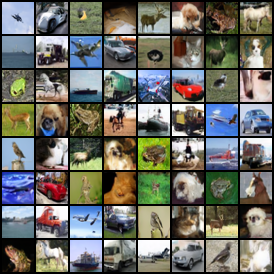
\includegraphics[width=\linewidth]{figures/cifar_flow/metrics_ddpm_cosine_vpred_raw_cfg25_5k_preview.png}
    \caption{5k metric preview}
  \end{subfigure}
  \caption{DDPM/DDIM 成为 CIFAR-10 最强定量结果。}
\end{figure}

\begin{table}[H]
  \centering
  \caption{CIFAR-10 最终定量结果}
  \begin{tabular}{lccccc}
    \toprule
    模型 & Sampler & Samples & CFG & FID & IS \\
    \midrule
    DDPM cosine v-pred U-Net & DDIM 250 & 5000 & 2.5 & 13.37 & 5.29 $\pm$ 0.14 \\
    EDM U-Net & Heun 40 & 1000 & 2.0 & 41.50 & 5.01 $\pm$ 0.48 \\
    \bottomrule
  \end{tabular}
\end{table}

\paragraph{困难与解决}
DDPM 分支需要明确 schedule、prediction type、DDIM steps 和 CFG scale。通过 cosine v-prediction 与 500 epoch 训练，最终显著优于前面的 Rectified Flow 展示图。

\paragraph{消融结论}
cosine schedule + v-prediction 是当前 CIFAR-10 最强配置；DDIM 250 + CFG 2.5 在质量和计算成本之间取得较好平衡。

\subsection{阶段 E：EDM 与 Visual64 展示}

\paragraph{方法与改进}
EDM 分支引入预条件化、连续噪声尺度和 Karras Heun sampler。CIFAR-10 EDM 用于测试是否能超过 DDPM/DDIM；Visual64 Pets EDM 用于获得更清晰、更适合 README 的视觉展示。

\paragraph{关键代码}
\begin{itemize}
  \item \code{src/edm.py}
  \item \code{labs/lab_cifar_flow/train_cifar10_edm_unet.py}
  \item \code{labs/lab_cifar_flow/sample_cifar10_edm.py}
  \item \code{labs/lab_visual64/train_visual64_edm_unet.py}
  \item \code{labs/lab_visual64/eval_visual64_sampling_sweep.py}
  \item \code{configs/visual64_pets_binary_edm_300ep.yaml}
\end{itemize}

\begin{figure}[H]
  \centering
  \begin{subfigure}{0.48\linewidth}
    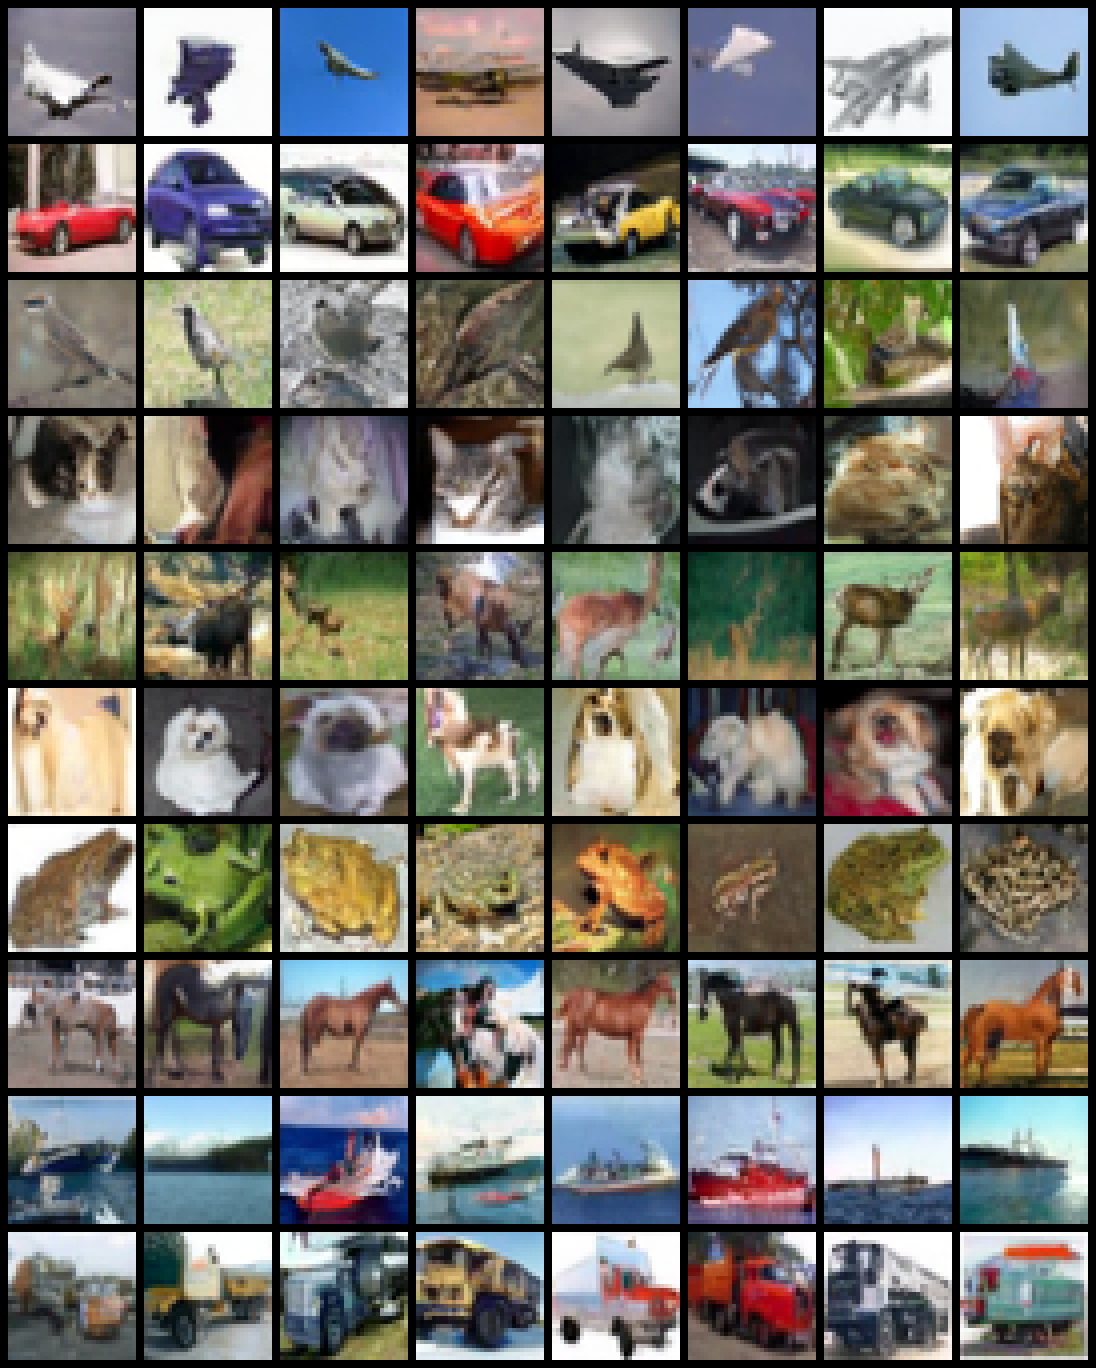
\includegraphics[width=\linewidth]{figures/cifar_flow/edm_cifar10_resume_300ep_heun40_cfg2_upscaled.png}
    \caption{CIFAR-10 EDM 300ep}
  \end{subfigure}
  \begin{subfigure}{0.48\linewidth}
    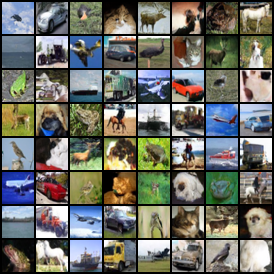
\includegraphics[width=\linewidth]{figures/cifar_flow/metrics_edm_resume_300ep_1k_preview.png}
    \caption{EDM metric preview}
  \end{subfigure}
  \caption{CIFAR-10 EDM 相比早期 EDM 更连贯，但未超过 DDPM/DDIM。}
\end{figure}

\begin{figure}[H]
  \centering
  \begin{subfigure}{0.48\linewidth}
    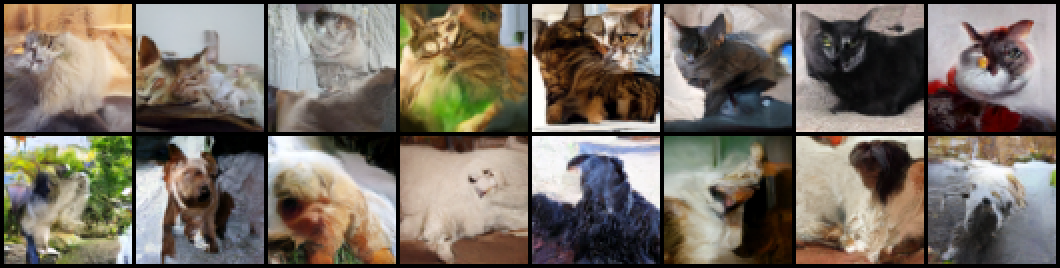
\includegraphics[width=\linewidth]{figures/visual64/visual64_best_binary_pets_heun80_cfg2.png}
    \caption{Binary Pets}
  \end{subfigure}
  \begin{subfigure}{0.48\linewidth}
    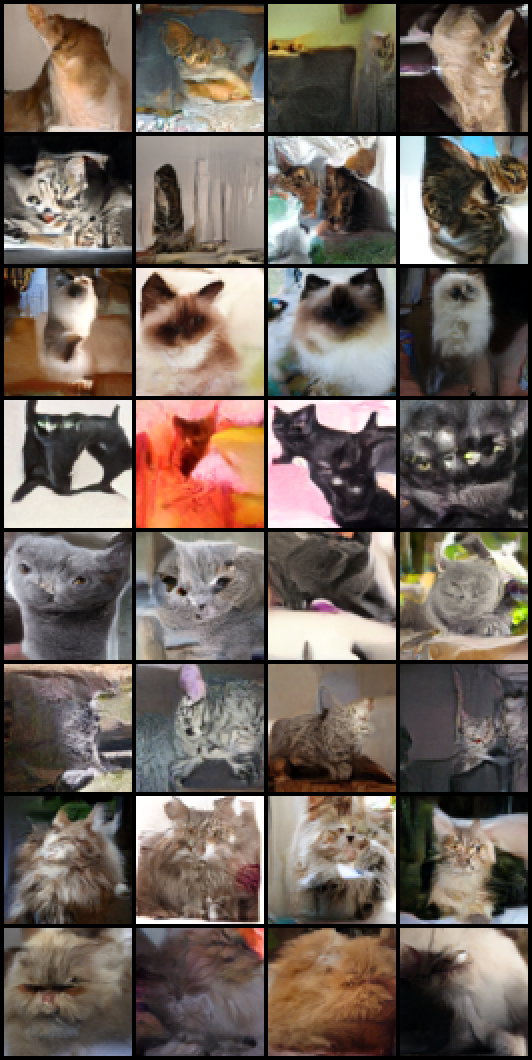
\includegraphics[width=\linewidth]{figures/visual64/visual64_best_37class_pets_heun80_cfg2.png}
    \caption{37-class Pets}
  \end{subfigure}
  \caption{Visual64 Pets EDM 是当前最清晰的视觉结果。}
\end{figure}

\begin{figure}[H]
  \centering
  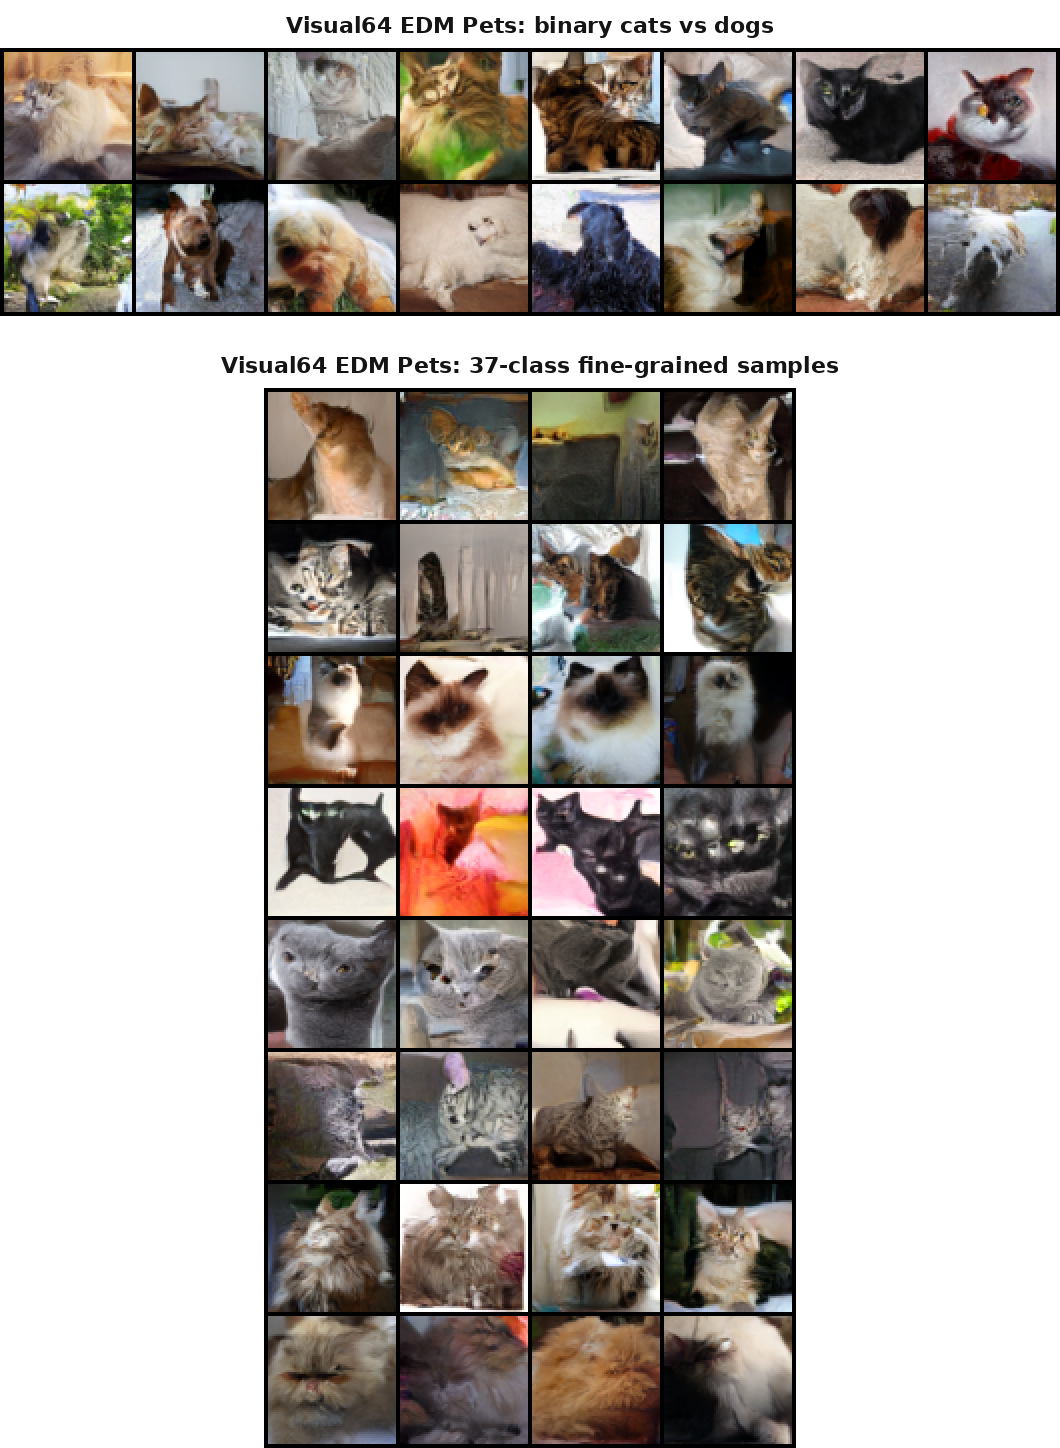
\includegraphics[width=0.95\linewidth]{figures/visual64/final_visual64_showcase_panel.png}
  \caption{最终展示图：Visual64 Pets EDM，Heun 80 steps，CFG 2.0。}
\end{figure}

\paragraph{困难与解决}
CIFAR-10 32x32 图像本身展示冲击力有限，EDM 定量也没有超过 DDPM/DDIM。解决方式是保留 DDPM/DDIM 作为 CIFAR-10 metric 主结果，同时用 64x64 Pets EDM 作为视觉主展示。

\paragraph{消融结论}
Visual64 sampling sweep 显示 CFG 2.0 和 Heun 80 steps 更稳；CFG 3.0 没有明显收益且更容易牺牲自然度；30/50 steps 可用，但 80 steps 细节更稳定。

\section{最终结果展示与结论}

\begin{table}[H]
  \centering
  \caption{最终项目交付物}
  \begin{tabular}{p{0.24\linewidth}p{0.32\linewidth}p{0.34\linewidth}}
    \toprule
    模块 & 代表文件 & 结论 \\
    \midrule
    课程 Lab & \code{labs/lab1}--\code{labs/lab5} & 完成从 ODE/SDE 到离散扩散的理论与代码闭环。 \\
    Mini-DiT & \code{src/dit/}, \code{labs/lab_dit} & 完成 patchify、AdaLN DiTBlock、MNIST 训练与 U-Net 对比。 \\
    CIFAR Rectified Flow & \code{src/image_flow_matching.py} & 适合研究 velocity、NFE、solver、guidance，但最终图像仍偏糊。 \\
    CIFAR DDPM/DDIM & \code{train_cifar10_ddpm_unet.py} & 最强 CIFAR-10 定量结果：FID 13.37，IS 5.29。 \\
    CIFAR/Visual EDM & \code{src/edm.py}, \code{labs/lab_visual64} & Visual64 Pets EDM 是最清晰的展示结果。 \\
    \bottomrule
  \end{tabular}
\end{table}

\begin{tcolorbox}[colback=papergray,colframe=paperblue,title=\textbf{最终判断},arc=1mm]
项目最终形成了清晰的研究叙事：先用课程 Lab 建立统一理论，再用 CIFAR-10 Rectified Flow 验证 velocity field 与 ODE sampling，发现图像质量瓶颈后通过 EMA、attention、time sampling 和 loss weighting 改进；当 Rectified Flow 仍不足以达到最终展示效果时，转向 DDPM/DDIM 与 EDM。最终保留 DDPM/DDIM 作为 CIFAR-10 定量主结果，Visual64 EDM 作为视觉主结果。
\end{tcolorbox}

\section*{复现实验入口}

\begin{lstlisting}[language=bash]
# CIFAR-10 final DDPM/DDIM samples
conda run -n fm_diffusion python labs/lab_cifar_flow/sample_cifar10_ddpm.py \
  --config configs/cifar10_final_showcase_cosine_vpred_upscaled.yaml

# CIFAR-10 final metrics
conda run -n fm_diffusion python labs/lab_cifar_flow/eval_cifar10_ddpm_metrics.py \
  --config configs/cifar10_metrics_final_cosine_vpred_5k.yaml

# Visual64 final panel
python labs/lab_visual64/make_final_visual64_showcase.py
\end{lstlisting}

\end{document}
